%LaTex cheat sheet template
\documentclass[10pt,a4paper,landscape]{article}

\usepackage[utf8]{inputenc}
\usepackage{amsmath}
\usepackage{xfrac}
\usepackage{empheq}
% \usepackage{amsfonts}
% \usepackage{amssymb}
% \usepackage{polynom}
\usepackage{multicol}
\usepackage{geometry}
% \usepackage{lipsum}
\usepackage{titlesec}
\usepackage[nodisplayskipstretch]{setspace}
% \usepackage{enumitem}
% \usepackage{wrapfig}
\usepackage{float}
\usepackage{graphicx}
% \usepackage{needspace}
\usepackage[table]{xcolor}
\usepackage{tcolorbox}
\usepackage{booktabs}
\usepackage{pdfpages}


\geometry{a4paper, left=0mm, top=0mm, right=0mm, bottom=2mm}

\titlespacing{\section}{0pt}{0pt}{0pt}
\titlespacing{\subsection}{0pt}{0pt}{0pt}
\titlespacing{\subsubsection}{0pt}{0pt}{0pt}

\setlength{\abovedisplayskip}{0pt}
\setlength{\belowdisplayskip}{0pt}
\setlength{\parindent}{0pt}

% \newcommand{\dropsign}[1]{\smash{\llap{\raisebox{-.5\normalbaselineskip}{$#1$\hspace{2\arraycolsep}}}}}

\begin{document}
\begin{multicols*}{3}
    \section*{Formulaire PartDiff}
    \subsection*{Généralités}
\textbf{Notations:}
\begin{align*}
    \frac{\partial u}{\partial y}     & = u_y    & \frac{\partial^2 u}{\partial y^2}         & = u_{yy} \\
    \frac{\partial^2 u}{\partial x^2} & = u_{xx} & \frac{\partial^2 u}{\partial x\partial y} & = u_{xy}
\end{align*}
\textbf{Condition de linéarité:}
\begin{subequations}
    \begin{equation*}
        \mathcal{L}(u+v)=\mathcal{L}(u)+\mathcal{L}(v)
    \end{equation*}
    \begin{equation*}
        \mathcal{L}(cu)=c\mathcal{L}(u)
    \end{equation*}
\end{subequations}
Si $\mathcal{L}u=0$ : \textit{linéaire homogène} \\
Si $\mathcal{L}u=f$ : \textit{linéaire inhomogène}\\
\textbf{Divergence:}\\
Pour un champ vectorielle $\overrightarrow{v}(x,y,z)=\begin{pmatrix} v_1(x,y,z) \\ v_2(x,y,z) \\ v_3(x,y,z) \end{pmatrix}$:
\begin{equation*}
    \text{div}(\overrightarrow{v})=\nabla\cdot\overrightarrow{v}=\frac{\partial v_1}{\partial x}+\frac{\partial v_2}{\partial y}+\frac{\partial v_3}{\partial z}
\end{equation*}
\textbf{Gradient:}\\
Pour un champ scalaire $u(x,y,z)$:
\begin{equation*}
    \text{grad}(u)=\nabla u=\begin{pmatrix} \frac{\partial u}{\partial x} \\ \frac{\partial u}{\partial y} \\ \frac{\partial u}{\partial z} \end{pmatrix}
\end{equation*}
\textbf{Rotationnel:}\\
\begin{equation*}
    \text{curl}(\overrightarrow{v}) = \nabla \times \overrightarrow{v} =
    \begin{pmatrix}
        \frac{\partial}{\partial x} \\
        \frac{\partial}{\partial y} \\
        \frac{\partial}{\partial z}
    \end{pmatrix}
    \times
    \begin{pmatrix}
        v_1(x,y,z) \\
        v_2(x,y,z) \\
        v_3(x,y,z)
    \end{pmatrix}
    =
    \begin{pmatrix}
        \frac{\partial v_3}{\partial y} - \frac{\partial v_2}{\partial z} \\
        \frac{\partial v_1}{\partial z} - \frac{\partial v_3}{\partial x} \\
        \frac{\partial v_2}{\partial x} - \frac{\partial v_1}{\partial y}
    \end{pmatrix}
\end{equation*}
\textbf{Laplacien}:
\begin{equation*}
    \Delta u=\text{div}(\Delta u)=u_{xx}+u_{yy}+u_{zz}
\end{equation*}
\textbf{Quelques propriétés:}
\begin{equation*}
    \text{div}(u\cdot \overrightarrow{v})=\overrightarrow{v}\cdot\nabla u+u\cdot\text{div}(\overrightarrow{v})
\end{equation*}
\textbf{Conditions initiales et aux bords:}\\
$u(x,t_0)=\phi(x)$ (diffusion, flux de chaleur)\\
$u(x,t_0)=\phi(x)$ et $u_t(x,t_0)=\psi(x)$ (ondes)\\
$u$ est spécifié : \textit{Dirichlet}\\
$\frac{\partial u}{\partial n}$ est spécifié : \textit{Neumann}\\
$\alpha u+\beta\frac{\partial u}{\partial n}$ est spécifié : \textit{Robin}\\
\textbf{Quelques types d'EDO:}\\
\underline{Equation de transport:}
\begin{equation*}
    u_t+cu_x=0
\end{equation*}
\underline{Equation d'onde:}\\
Pour une onde se propageant dans la direction $x$:
\begin{equation*}
    u_{tt}=c^2u_{xx}
\end{equation*}\\
Pour une onde se propageant dans deux directions:
\begin{equation*}
    u_{tt}=c^2\Delta u=c^2(u_{xx}+u_{yy})
\end{equation*}
\underline{Equation de diffusion:}
\begin{equation*}
    u_t=ku_{xx}
\end{equation*}
\textbf{EDO connues:}
\begin{equation*}
    \begin{aligned}
         & x''+\beta^2x=0 \quad\rightarrow\quad x=A\cos(\beta t)+B\sin(\beta t) \\
         & x''-\beta^2x=0 \quad\rightarrow\quad x=Ce^{\beta t}+De^{-\beta t}    \\
         & =(C+D)\cosh(\beta t)+(C-D)\sinh(\beta t)                             \\
         & x''=0 \quad\rightarrow\quad x=Et+F                                   \\
         & x'\pm \beta x=0 \quad\rightarrow\quad x=Ge^{\mp\beta t}              \\
    \end{aligned}
\end{equation*}
\textbf{Taylor}\\
\underline{1D:}\\
Le développement de Taylor de $u(x)$ autour de $x_i$:
\begin{equation*}
    u(x)=u(x_i)+\frac{u'(x_i)}{1!}(x-x_i)+\frac{u''(x_i)}{2!}(x-x_i)^2+\frac{u'''(x_i)}{3!}(x-x_i)^3+\cdots
\end{equation*}
\underline{2D:}\\
Le développement de Taylor de $u(x,y)$ autour de $(x_i,y_i)$:
\begin{equation*}
    \begin{aligned}
        u(x,y) & =u(x_i,y_i)+(u_x+u_y)(x-x_i,y-y_i)                                     \\
               & +\frac{1}{2!}(u_{xx}+2u_{xy}+u_{yy})(x-x_i,y-y_i)^2                    \\
               & +\frac{1}{3!}(u_{xxx}+3u_{xxy}+3u_{xyy}+u_{yyy})(x-x_i,y-y_i)^3+\cdots
    \end{aligned}
\end{equation*}
\textbf{Max-norm:}
\begin{equation*}
    ||u||_{\infty}=\max_{x\in\Omega}|u(x)|
\end{equation*}


\columnbreak
\subsection*{EDP linéaire du premier ordre}
\textbf{Quelques équations simples:}
\begin{figure}[H]
    \centering
    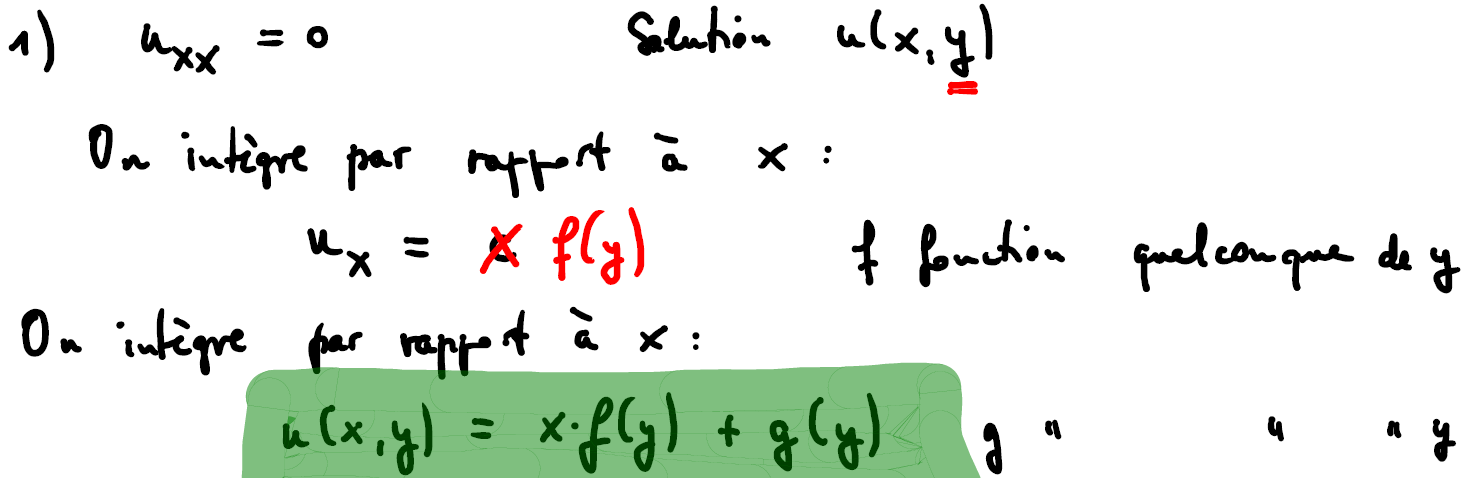
\includegraphics[width=\linewidth]{images/semain1_equ_simple1.png}
\end{figure}
\begin{figure}[H]
    \centering
    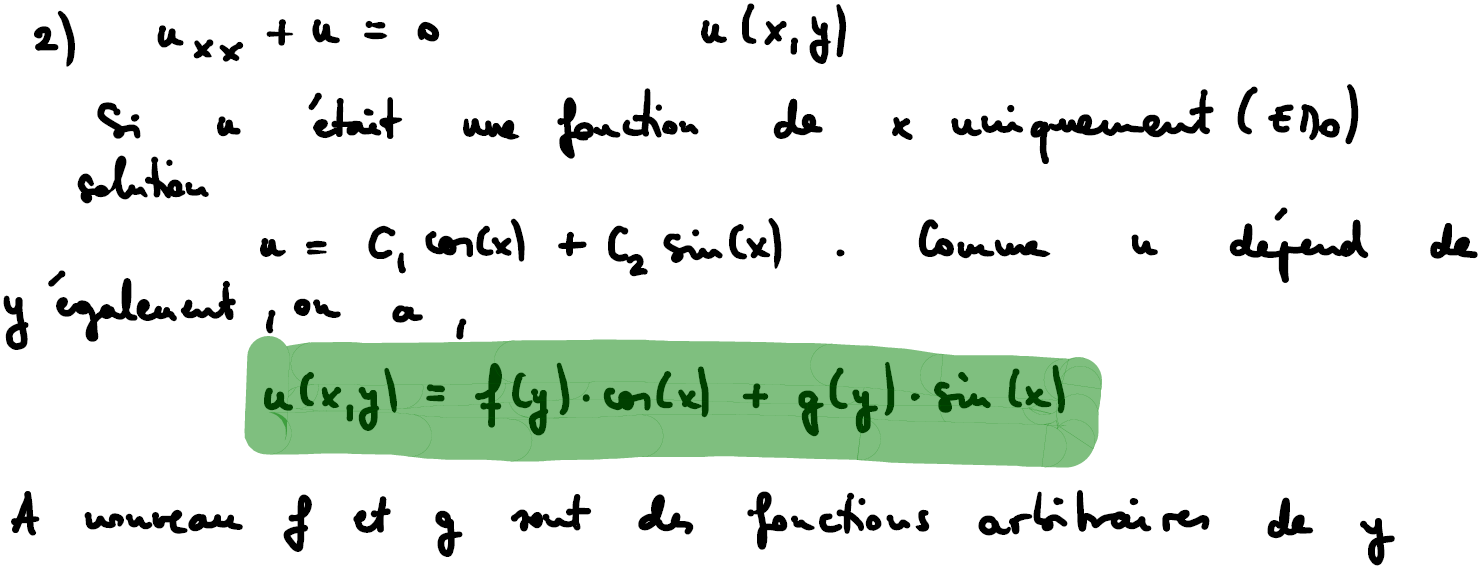
\includegraphics[width=\linewidth]{images/semain1_equ_simple2.png}
\end{figure}
\begin{figure}[H]
    \centering
    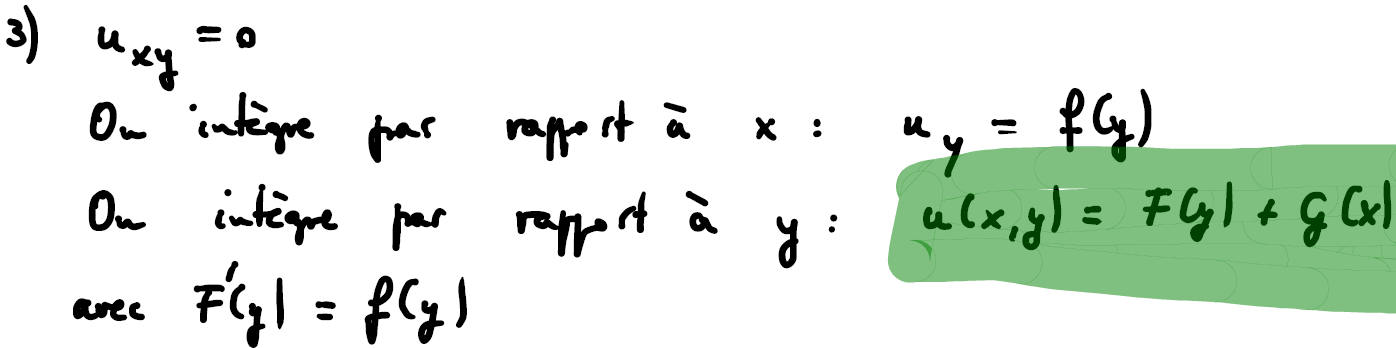
\includegraphics[width=\linewidth]{images/semain1_equ_simple3.png}
\end{figure}
\textbf{Equation à coefficients constants:}
\begin{subequations}
    \begin{equation*}
        au_x+bu_y=0
    \end{equation*}
    \begin{equation*}
        \boxed{u(x,y)=f(bx-ay)}
    \end{equation*}
\end{subequations}
\begin{figure}[H]
    \centering
    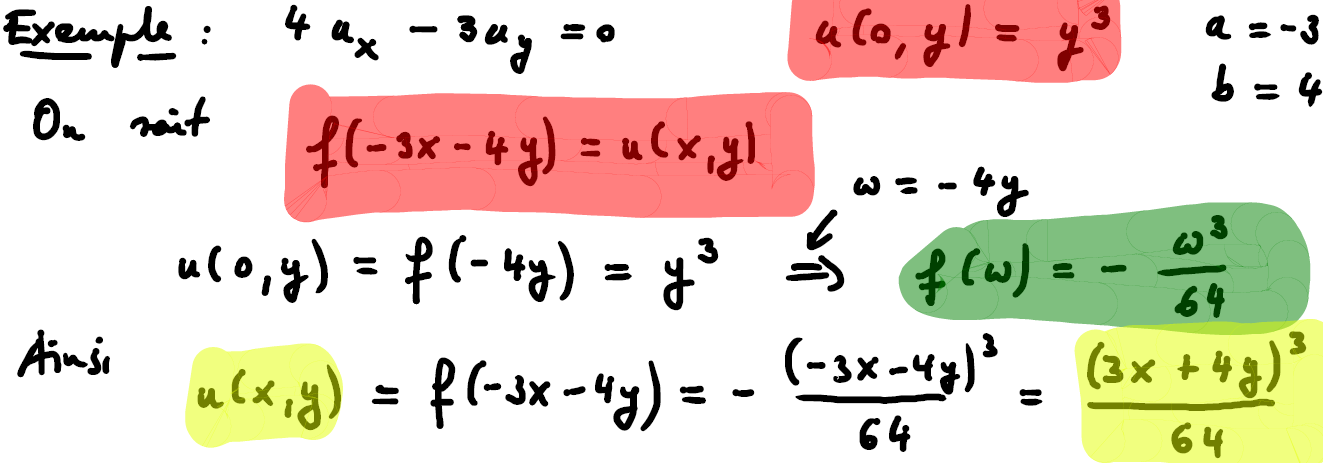
\includegraphics[width=\linewidth]{images/semaine1_equ_coeff_const.png}
\end{figure}
\textbf{Equation à coefficients variables:}
\begin{subequations}
    \begin{equation*}
        a(x,y)u_x+b(x,y)u_y=0
    \end{equation*}
    \begin{equation*}
        \boxed{\frac{\mathrm{d} y}{\mathrm{d} x}=\frac{b(x,y)}{a(x,y)}}
    \end{equation*}
\end{subequations}
\begin{figure}[H]
    \centering
    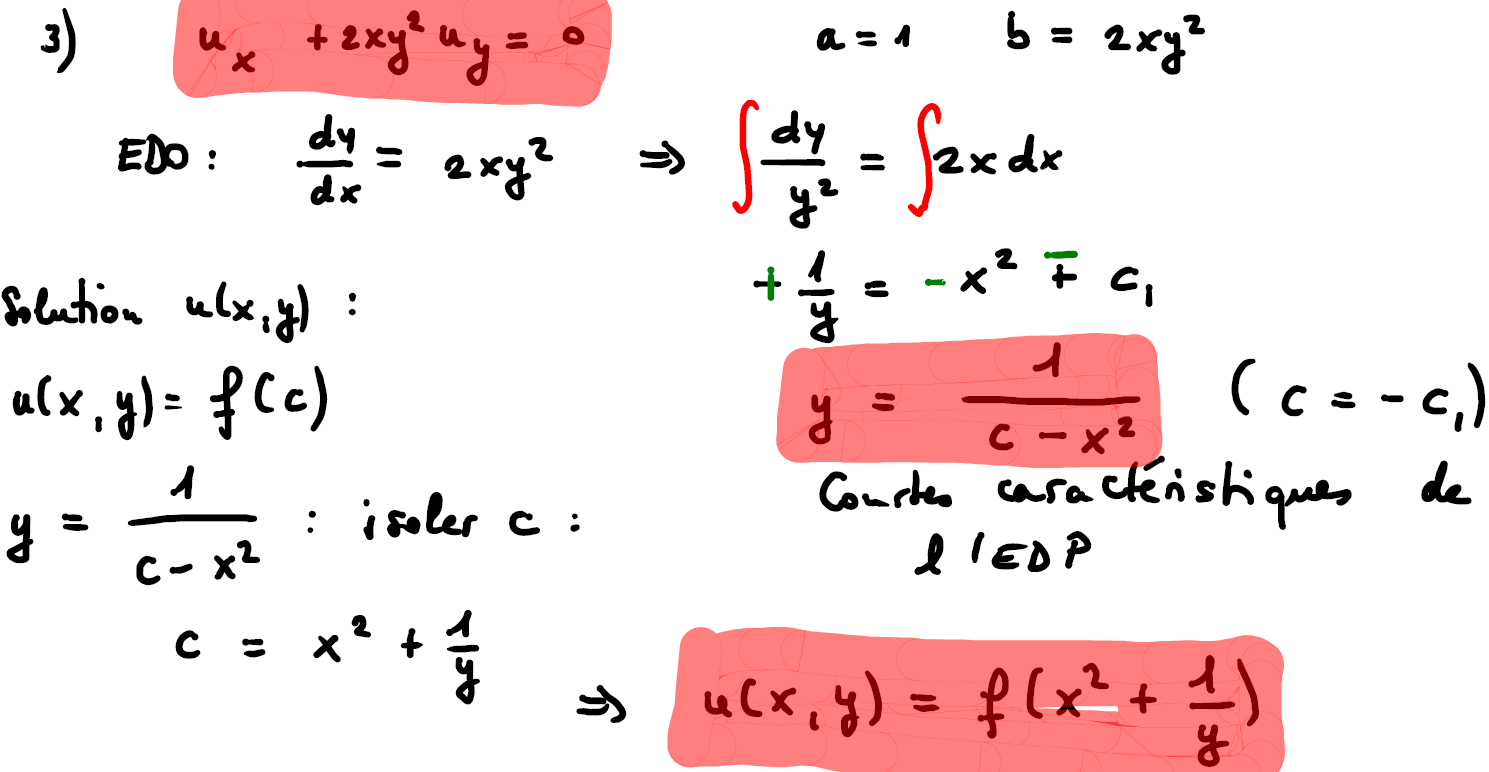
\includegraphics[width=\linewidth]{images/semaine1_equ_coeff_var1.png}
\end{figure}



\subsection*{EDP linéaire du second ordre}
\begin{equation*}
    Au_{xx}+Bu_{xy}+Cu_{yy}+Du_x+Eu_y+Fu=G
\end{equation*}
$A$, $B$, $C$, $D$, $E$, $F$, $G$ constantes ou des fonctions de $x$ et $y$.\\
\textit{Parabolique} si $B^2-4AC=0$\\
\textit{Hyperbolique} si $B^2-4AC>0$\\
\textit{Elliptique} si $B^2-4AC<0$\\
Trouver les régions de l'EDP:
\begin{equation*}
    yu_{xx}-2u_{xy}+xu_{yy}=0
\end{equation*}
\begin{figure}[H]
    \centering
    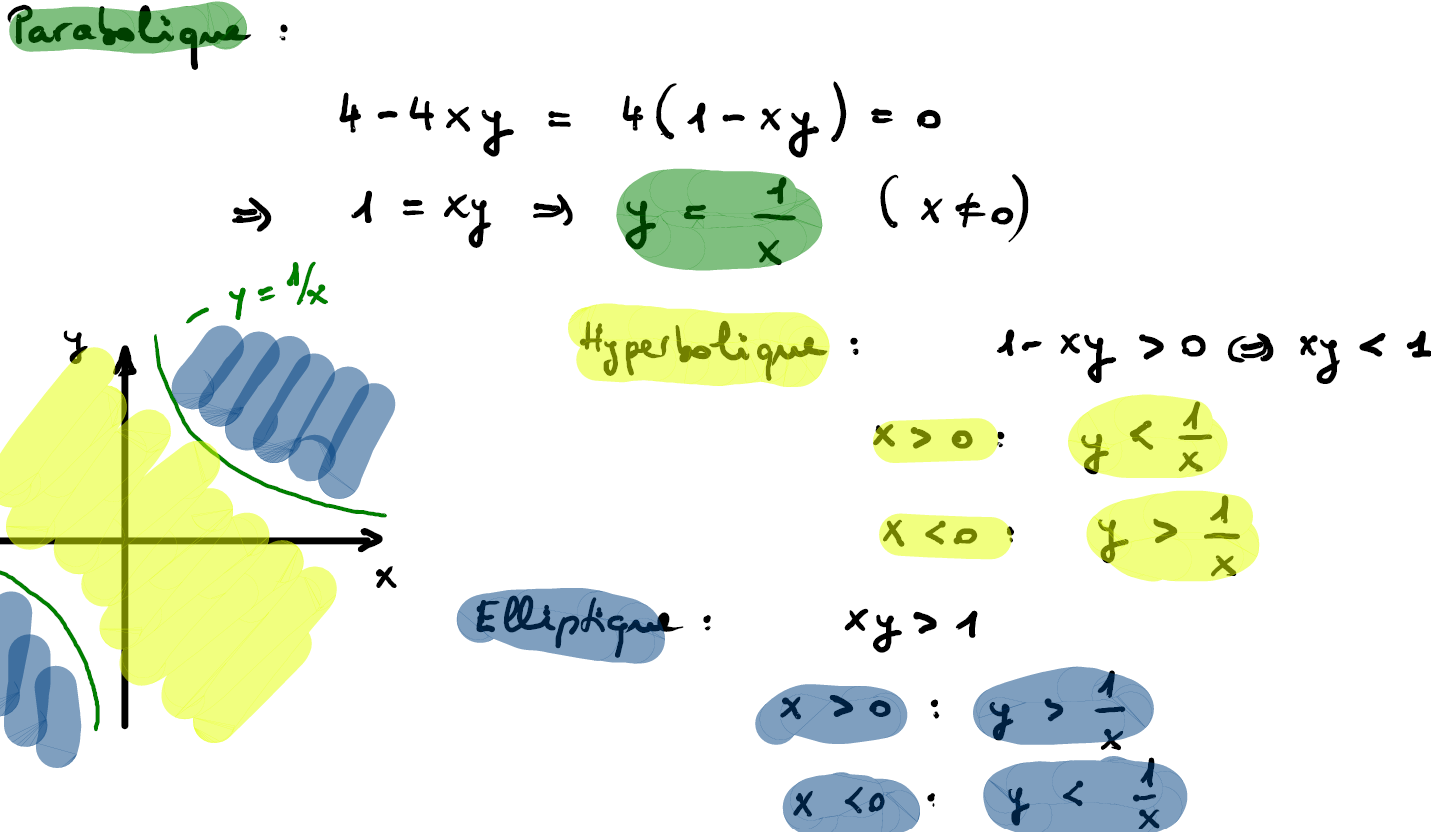
\includegraphics[width=\linewidth]{images/semaine2_edp_ordre2_classif.png}
\end{figure}




    %\columnbreak
    \subsection*{Equation d'onde}
\begin{equation*}
    u_{tt}=c^2u_{xx}
\end{equation*}
\textbf{Solution générale:}
\begin{equation*}
    \boxed{u(x,t)=f(x+ct)+g(x-ct)}
\end{equation*}
$f$ et $g$ sont deux fonction quelconques d'une seule variable.\\
\textbf{Solution avec condition initiales:}
\begin{equation*}
    \boxed{u(x,t)=\frac{1}{2}[\phi(x+ct)+\psi(x-ct)]+\frac{1}{2c}\int_{x-ct}^{x+ct}\psi(s)\mathrm{d}s}
\end{equation*}
\begin{figure}[H]
    \centering
    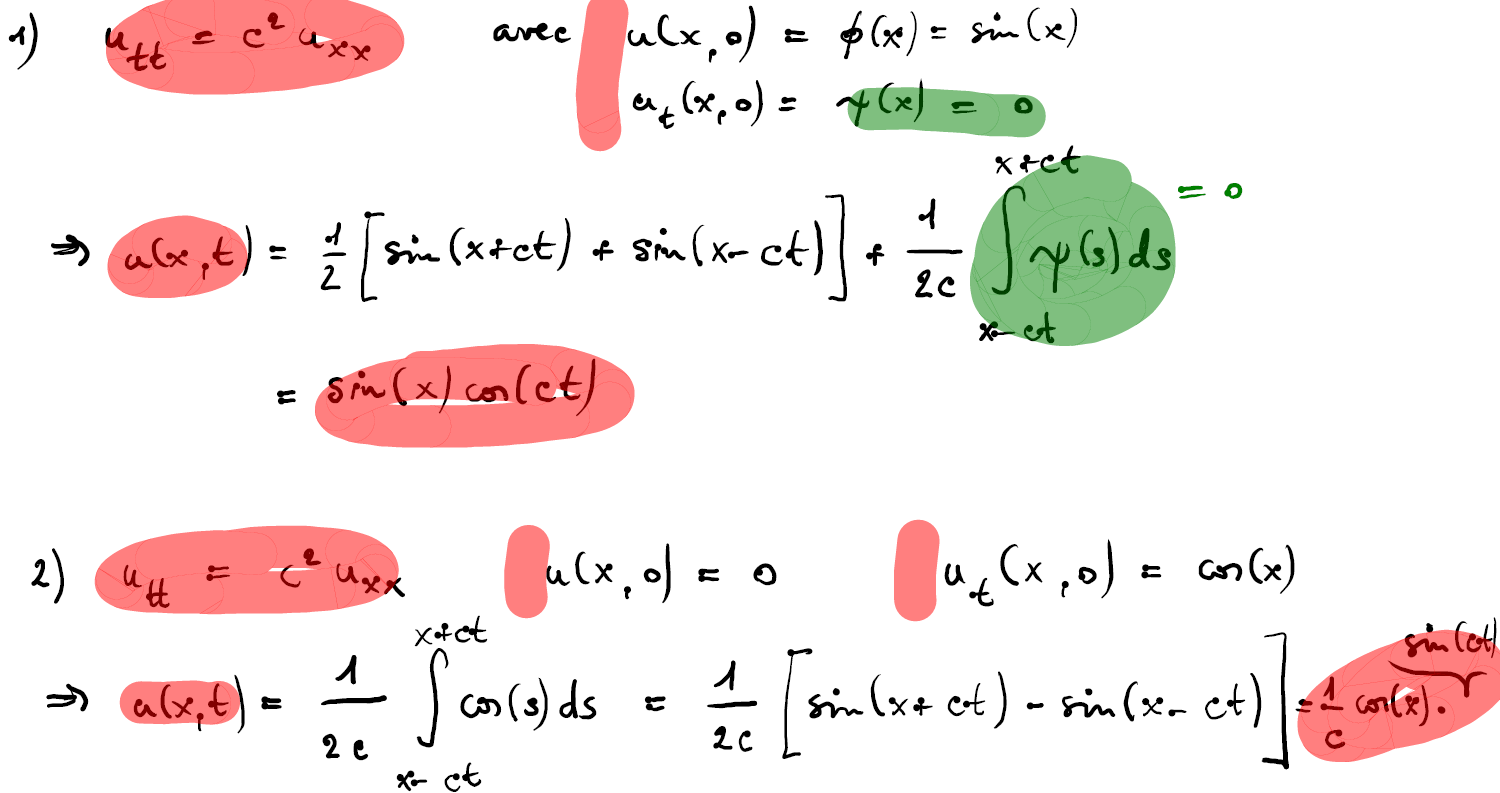
\includegraphics[width=\linewidth]{images/semaine2_onde.png}
\end{figure}
    \subsection*{Equation de diffusion}
\begin{equation*}
    u_t=ku_{xx}
\end{equation*}
\textbf{Principe du maximum:}\\
Si u(x, t) satisfait l'équation de diffusion dans un rectangle
(disons, $0 \leq x \leq l$, $0 \leq t \leq T$) dans l'espace-temps, alors la valeur
maximale de $u(x, t)$ est atteinte soit initialement ($t = 0$), soit sur
les côtés ($x = 0$ ou $x = l$)
\begin{figure}[H]
    \centering
    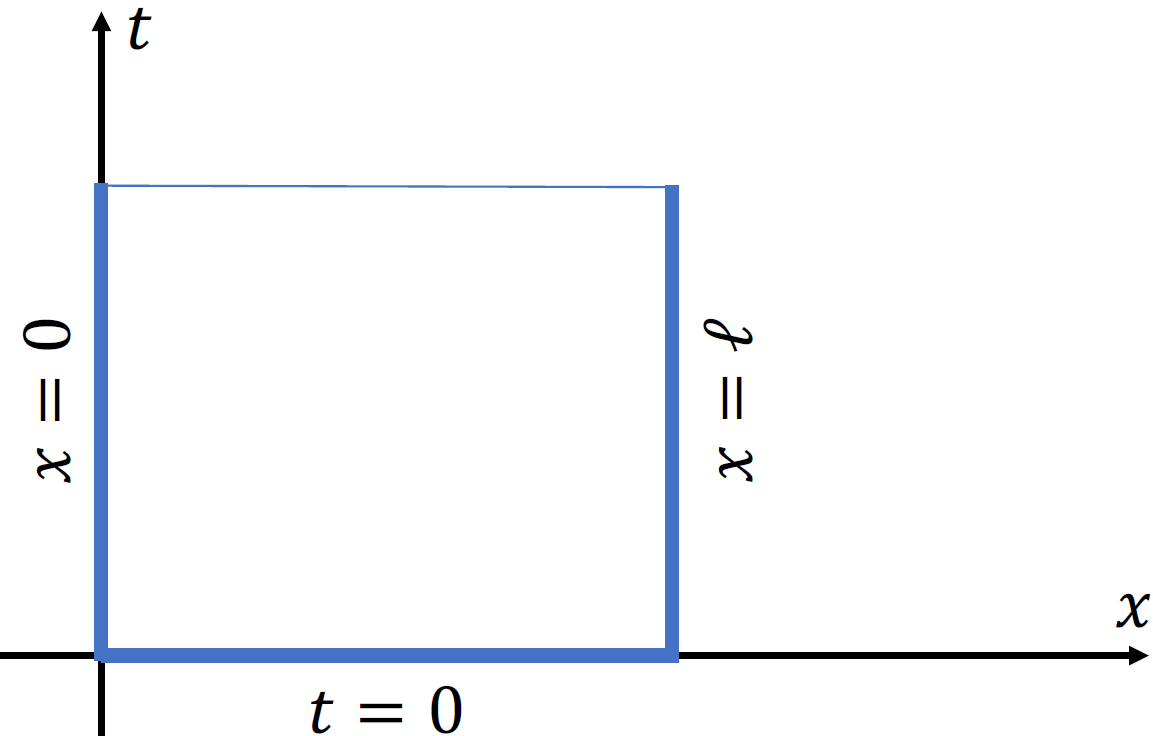
\includegraphics[width=0.5\linewidth]{images/semaine3_principe_max.png}
\end{figure}
La valeur minimale à la même propriété.\\
\textbf{Solution avec condition initiale:}
\begin{equation*}
    \boxed{u(x,t)=\frac{1}{2\sqrt{\pi kt}}\int_{-\infty}^{+\infty}e^{-\frac{(x-y)^2}{4kt}}\phi(y)\mathrm{d}y}
\end{equation*}
\textbf{Fonction d'erreur:}
\begin{subequations}
    \begin{equation*}
        \text{erf}(x)=\frac{2}{\sqrt{\pi}}\int_0^xe^{-p^2}\mathrm{d}p
    \end{equation*}
    \begin{equation*}
        \left\{
        \begin{aligned}
             & \int_{-\infty}^{\infty}e^{-p^2}\mathrm{d}p=\sqrt{\pi} \\
             & \int_{0}^{\infty}e^{-p^2}\mathrm{d}p=\frac{1}{2}
        \end{aligned}
        \right.
    \end{equation*}
\end{subequations}
Résoudre l'équation de diffusion avec la condition initiale:
\begin{equation*}
    \left\{
    \begin{aligned}
         & \phi(x)=1\quad\text{pour}\quad x>0 \\
         & \phi(x)=3\quad\text{pour}\quad x<0
    \end{aligned}
    \right.
\end{equation*}
\begin{figure}[H]
    \centering
    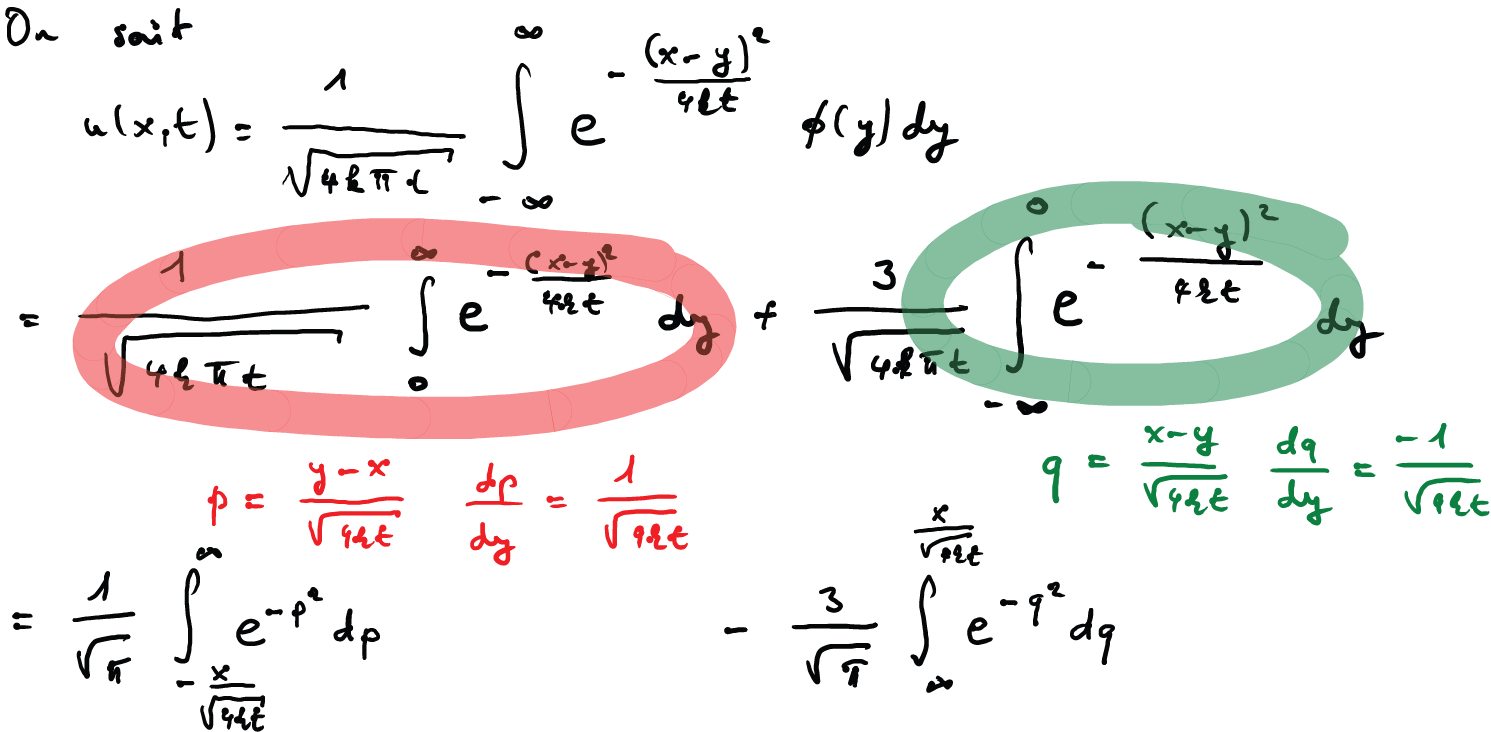
\includegraphics[width=\linewidth]{images/semaine3_diff1.png}
\end{figure}
\begin{figure}[H]
    \centering
    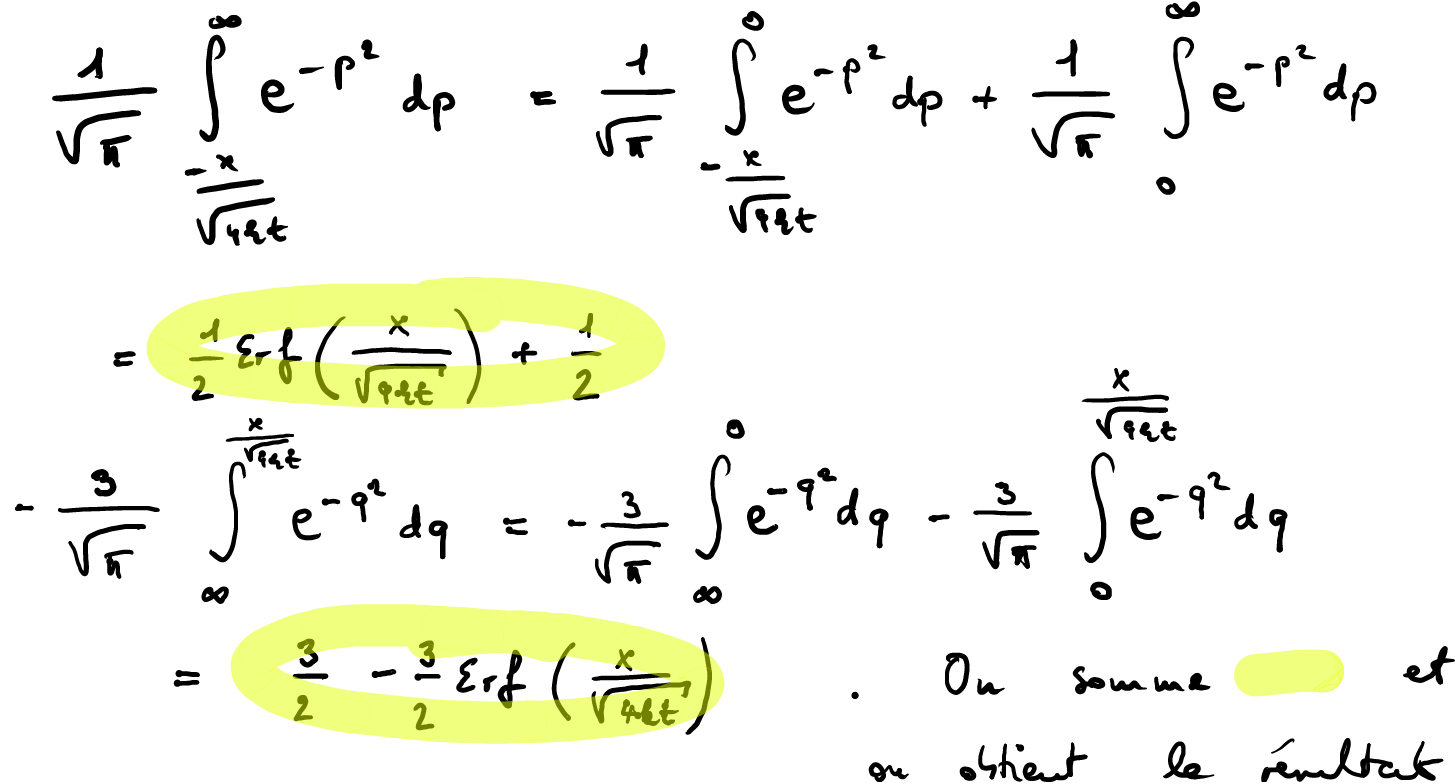
\includegraphics[width=\linewidth]{images/semaine3_diff2.png}
\end{figure}



    \subsection*{Problèmes bornés}
\textbf{Problème de Dirichlet:}\\
\underline{Onde:}
\begin{equation*}
    \left\{
    \begin{aligned}
         & u_{tt}=c^2u_{xx} \\
         & u(0,t)=u(l,t)=0  \\
         & u(x,0)=\phi(x)   \\
         & u_t(x,0)=\psi(x)
    \end{aligned}
    \right.
\end{equation*}
\begin{empheq}[box=\fbox]{gather*}
    u(x,t)=\sum_{n=1}^{\infty}\left[A_n\cos\left(\frac{n\pi c}{l}t\right)+B_n\sin\left(\frac{n\pi c}{l}t\right)\right]\sin\left(\frac{n\pi}{l}x\right) \\
    \phi(x)=\sum_{n=1}^{\infty}A_n\sin\left(\frac{n\pi}{l}x\right) \\
    \psi(x)=\sum_{n=1}^{\infty}\frac{n\pi c}{l}B_n\sin\left(\frac{n\pi}{l}x\right)
\end{empheq}
\underline{Diffusion:}
\begin{equation*}
    \left\{
    \begin{aligned}
         & u_t=ku_{xx}     \\
         & u(0,t)=u(l,t)=0 \\
         & u(x,0)=\phi(x)
    \end{aligned}
    \right.
\end{equation*}
\begin{empheq}[box=\fbox]{gather*}
    u(x,t)=\sum_{n=1}^{\infty}A_ne^{-\left(\frac{n\pi}{l}\right)^2kt}\sin\left(\frac{n\pi}{l}x\right) \\
    \phi(x)=\sum_{n=1}^{\infty}A_n\sin\left(\frac{n\pi}{l}x\right)
\end{empheq}
\textbf{Problème de Neumann:}\\
\underline{Onde:}
\begin{equation*}
    \left\{
    \begin{aligned}
         & u_{tt}=c^2u_{xx}    \\
         & u_x(0,t)=u_x(l,t)=0 \\
         & u(x,0)=\phi(x)      \\
         & u_t(x,0)=\psi(x)
    \end{aligned}
    \right.
\end{equation*}
\begin{empheq}[box=\fbox]{gather*}
    \begin{split}
        u(x,t) &=  \frac{1}{2}A_0+\frac{1}{2}B_0t\\
        & +\sum_{n=1}^{\infty}\left[A_n\cos\left(\frac{n\pi c}{l}t\right)+B_n\sin\left(\frac{n\pi c}{l}t\right)\right]\cos\left(\frac{n\pi}{l}x\right)
    \end{split}\\
    \phi(x)=\frac{1}{2}A_0+\sum_{n=1}^{\infty}A_n\cos\left(\frac{n\pi}{l}x\right) \\
    \psi(x)=\frac{1}{2}B_0+\sum_{n=1}^{\infty}\frac{n\pi c}{l}B_n\cos\left(\frac{n\pi}{l}x\right)
\end{empheq}
\underline{Diffusion:}
\begin{equation*}
    \left\{
    \begin{aligned}
         & u_t=ku_{xx}         \\
         & u_x(0,t)=u_x(l,t)=0 \\
         & u(x,0)=\phi(x)
    \end{aligned}
    \right.
\end{equation*}
\begin{empheq}[box=\fbox]{gather*}
    u(x,t)=\frac{1}{2}A_0+\sum_{n=1}^{\infty}A_ne^{-\left(\frac{n\pi}{l}\right)^2kt}\cos\left(\frac{n\pi}{l}x\right) \\
    \phi(x)=\frac{1}{2}A_0+\sum_{n=1}^{\infty}A_n\cos\left(\frac{n\pi}{l}x\right)
\end{empheq}
\textbf{Valeurs propres et fonctions propres:}\\
\underline{Exemple:}\\
Résoudre avec les conditions Dirichlet:
\begin{equation*}
    u_t=ju_{xx}
\end{equation*}
\begin{figure}[H]
    \centering
    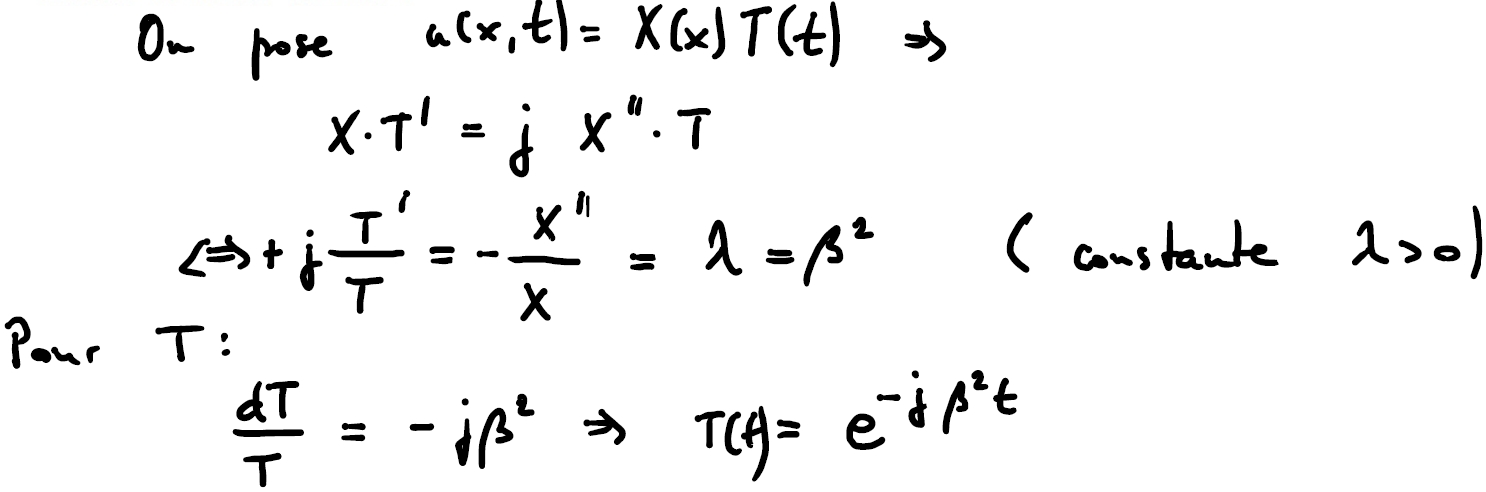
\includegraphics[width=\linewidth]{images/semaine4_val_vect_propre1.png}
\end{figure}
\begin{figure}[H]
    \centering
    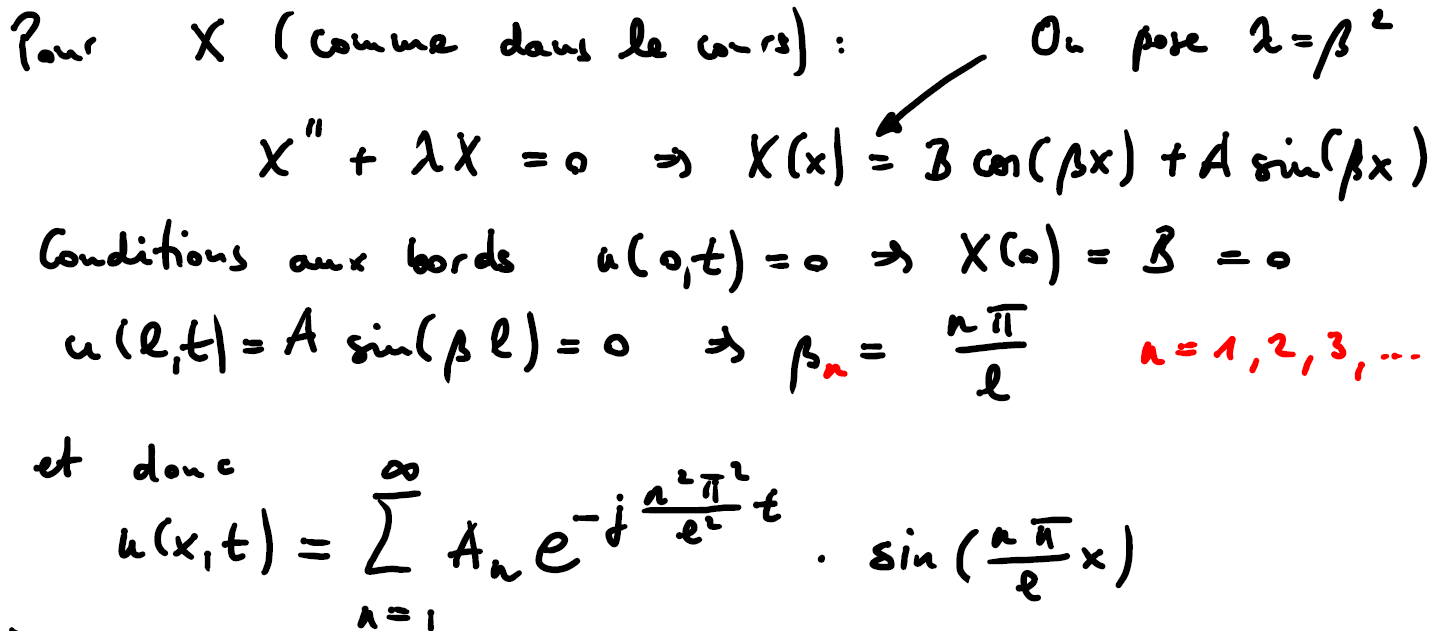
\includegraphics[width=\linewidth]{images/semaine4_val_vect_propre2.png}
\end{figure}
Dans ce cas-ci, la valeur propre est $\lambda=\beta^2=\frac{n^2\pi^2}{l^2}$ trouvée en
résolvant $\frac{-X''}{X}=\lambda$ et la fonction propre est $T(t)=e^{-j\beta^2t}$
trouvée en résolvant $j\frac{T'}{T}=\lambda$.\\
\underline{Conditions mixte}\\
\begin{equation*}
    \lambda=\frac{(n+\sfrac{1}{2})^2\pi^2}{l^2}
\end{equation*}
La fonction propre est elle à calculer selon les conditions au bord spécifiées.\\


    \subsection*{Fonctions harmoniques}
Résolution similaire aux problèmes bornés.\\
\textbf{Exemple:}\\
On veut résoudre:
\begin{equation*}
    \left\{
    \begin{aligned}
         & u(x,y)=\Delta u=u_{xx}+u_{yy} \\
         & D=\{0<x<a,0<y<b\}             \\
    \end{aligned}
    \right.
\end{equation*}
avec les conditions aux bords:
\begin{figure}[H]
    \centering
    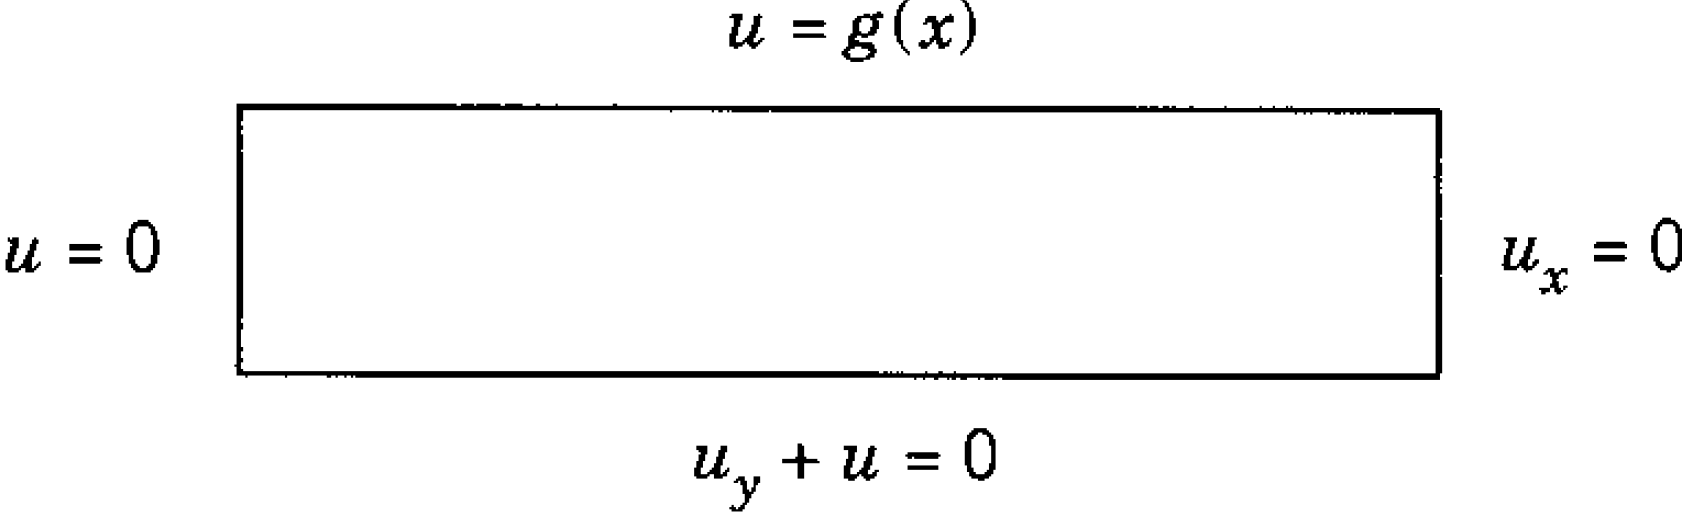
\includegraphics[width=0.75\linewidth]{images/semaine5_condi_bord.png}
\end{figure}
trouver les valeurs propres et les fonctions propres :
\begin{subequations}
    \begin{equation*}
        u(x,y)=X(x)Y(y)\Longrightarrow \frac{X''}{X}+\frac{Y''}{Y}=0
    \end{equation*}
    \begin{equation*}
        \left\{
        \begin{aligned}
             & X''+\lambda X=0 \quad \text{pour} \quad 0\leq x\leq a \\
             & Y''-\lambda Y=0 \quad \text{pour} \quad 0\leq x\leq b \\
        \end{aligned}
        \right.
    \end{equation*}
    \begin{equation*}
        \left\{
        \begin{aligned}
             & \lambda=\beta^2=(n+\sfrac{1}{2})^2\frac{\pi^2}{a^2}                                       \\
             & \colorbox{green}{$X(x)$}=A\cos(\beta x)+B\sin(\beta x)=\colorbox{green}{$B\sin(\beta x)$} \\
             & \text{car} \quad X(0)=X'(a)=0
        \end{aligned}
        \right.
    \end{equation*}
    \begin{equation*}
        \left\{
        \begin{aligned}
             & \colorbox{yellow}{$Y(y)$}=A\cosh(\beta y)+B\sinh(\beta y)=\colorbox{yellow}{$\beta\cosh(\beta y)-\sinh(\beta y)$} \\
             & \text{car} \quad Y'(0)+Y(0)=C+D\beta=0 \Longrightarrow D=-1 \quad \text{et} \quad C=\beta                         \\
        \end{aligned}
        \right.
    \end{equation*}
\end{subequations}
il reste à sommer la série est trouver $g(x)$
\begin{subequations}
    \begin{equation*}
        u(x,y)=\sum_{n=0}^{\infty}\colorbox{green}{$B_n\sin(\beta_nx)$}\colorbox{yellow}{$(\beta_n\cosh(\beta_ny)-\sinh(\beta_ny))$}
    \end{equation*}
    \begin{equation*}
        u(x,b)=g(x)=\sum_{n=0}^{\infty}\underbrace{B_n(\beta_n\cosh(\beta_nb)-\sinh(\beta_nb))}_{E_n}\sin(\beta_nx)
    \end{equation*}
\end{subequations}
\textbf{Formule de poissons:}\\
On veut séparer les variables en coordonnées polaires $u=R(r)\Theta(\theta)$:
\begin{equation*}
    u_{xx}=+u_{yy}=u_{rr}+\frac{1}{r}u_r+\frac{1}{r^2}u_{\theta\theta}
\end{equation*}
puis on procède comme d'habitude.

    \subsection*{Calcul des coefficients de Fourier:}
\textbf{Série en sinus - Dirichlet}\\
\underline{Pour l'équation de diffusion:}
\begin{equation*}
    \boxed{A_n=\frac{2}{l}\int_0^l\phi(x)\sin\left(\frac{n\pi}{l}x\right)\mathrm{d}x}\quad n=1,2,\cdots
\end{equation*}
\underline{Pour l'équation d'onde:}
\begin{subequations}
    \begin{equation*}
        \boxed{A_n=\frac{2}{l}\int_0^l\phi(x)\sin\left(\frac{n\pi}{l}x\right)\mathrm{d}x}\quad n=1,2,\cdots
    \end{equation*}
    \begin{equation*}
        \boxed{\frac{n\pi c}{l}B_n=\frac{2}{l}\int_0^l\psi(x)\sin\left(\frac{n\pi}{l}x\right)\mathrm{d}x}\quad n=1,2,\cdots
    \end{equation*}
\end{subequations}
\textbf{Série en cosinus - Neumann:}\\
\underline{Pour l'équation de diffusion:}
\begin{equation*}
    \boxed{A_n=\frac{2}{l}\int_0^l\phi(x)\cos\left(\frac{n\pi}{l}x\right)\mathrm{d}x}\quad n=0,1,2,\cdots
\end{equation*}
\underline{Pour l'équation d'onde:}
\begin{subequations}
    \begin{equation*}
        \boxed{A_n=\frac{2}{l}\int_0^l\phi(x)\cos\left(\frac{n\pi}{l}x\right)\mathrm{d}x}\quad n=0,1,2,\cdots
    \end{equation*}
    \begin{equation*}
        \boxed{B_0=\frac{2}{l}\int_0^l\psi(x)\mathrm{d}x}
    \end{equation*}
    \begin{equation*}
        \boxed{\frac{n\pi c}{l}B_n=\frac{2}{l}\int_0^l\psi(x)\cos\left(\frac{n\pi}{l}x\right)\mathrm{d}x}\quad n=1,2,\cdots
    \end{equation*}
\end{subequations}
\textbf{Série en cosinus et sinus - périodique:}
\begin{subequations}
    \begin{equation*}
        \boxed{A_n=\frac{1}{l}\int_{-l}^l\phi(x)\cos\left(\frac{n\pi}{l}x\right)\mathrm{d}x} \quad n=0,1,2,\cdots
    \end{equation*}
    \begin{equation*}
        \boxed{B_n=\frac{1}{l}\int_{-l}^l\phi(x)\sin\left(\frac{n\pi}{l}x\right)\mathrm{d}x} \quad n=1,2,\cdots
    \end{equation*}
\end{subequations}


    \pagebreak
    \subsection*{Laplace}
\textbf{Table des transformées de Laplace:}
\begin{center}
    \renewcommand{\arraystretch}{1.25}
    \begin{tabular}{cc}
        \toprule
        $f(t)$                                            & $F(s)$                                   \\
        \midrule
        $H(t)$                                            & $\frac{1}{s}$                            \\
        $t$                                               & $\frac{1}{s^2}$                          \\
        $t^n$                                             & $\frac{n!}{s^{n+1}}$                     \\
        $\sqrt{t}$                                        & $\frac{1}{2}\sqrt{\pi}s^{-\sfrac{3}{2}}$ \\
        $\frac{1}{\sqrt{t}}$                              & $\sqrt{\pi}s^{-\sfrac{1}{2}}$            \\
        $e^{at}$                                          & $\frac{1}{s-a}$                          \\
        $\sin(\omega t)$                                  & $\frac{\omega}{s^2+\omega^2}$            \\
        $\cos(\omega t)$                                  & $\frac{s}{s^2+\omega^2}$                 \\
        $\sinh(at)$                                       & $\frac{a}{s^2-a^2}$                      \\
        $\cosh(at)$                                       & $\frac{s}{s^2-a^2}$                      \\
        $H(t-b)$                                          & $\frac{e^{-bs}}{s}$                      \\
        $\delta(t-b)$                                     & $e^{-bs}$                                \\
        $a(4\pi t^3)^{-\sfrac{1}{2}}e^{-\sfrac{a^2}{4t}}$ & $e^{a\sqrt{s}}$                          \\
        $(\pi t)^{-\sfrac{1}{2}}e^{-\sfrac{a^2}{4t}}$     & $\frac{1}{\sqrt{s}}e^{a\sqrt{s}}$        \\
        $1-\text{erf}\left(\frac{a}{\sqrt{4t}}\right)$    & $\frac{1}{s}e^{a\sqrt{s}}$               \\
        \bottomrule
    \end{tabular}
\end{center}
\textbf{Propriétés:}
\begin{center}
    \renewcommand{\arraystretch}{1.5}
    \begin{tabular}{cc}
        \toprule
        Fonction                                                & Transformée                                     \\
        \midrule
        $af(t)+bg(t)$                                           & $aF(s)+bG(s)$                                   \\
        $\frac{\mathrm{d}f}{\mathrm{d}t}$                       & $sF(s)-f(0)$                                    \\
        $\frac{\mathrm{d}^2f}{\mathrm{d}t^2}$                   & $s^2F(s)-sf(0)-f'(0)$                           \\
        $e^{bt}f(t)$                                            & $F(s-b)$                                        \\
        $\frac{f(t)}{t}$                                        & $\int_s^\infty F(\tilde{s})\mathrm{d}\tilde{s}$ \\
        $tf(t)$                                                 & $-\frac{\mathrm{d}F}{\mathrm{d}s}$              \\
        $H(t-b)f(t-b)$                                          & $e^{-bs}F(s)$                                   \\
        $f(ct)$                                                 & $\frac{1}{c}F\left(\frac{s}{c}\right)$          \\
        $\int_0^tg(t-\tilde{t})f(\tilde{t})\mathrm{d}\tilde{t}$ & $G(s)F(s)$                                      \\
        \bottomrule
    \end{tabular}
\end{center}
\columnbreak
\textbf{Exemples:}
\begin{figure}[H]
    \centering
    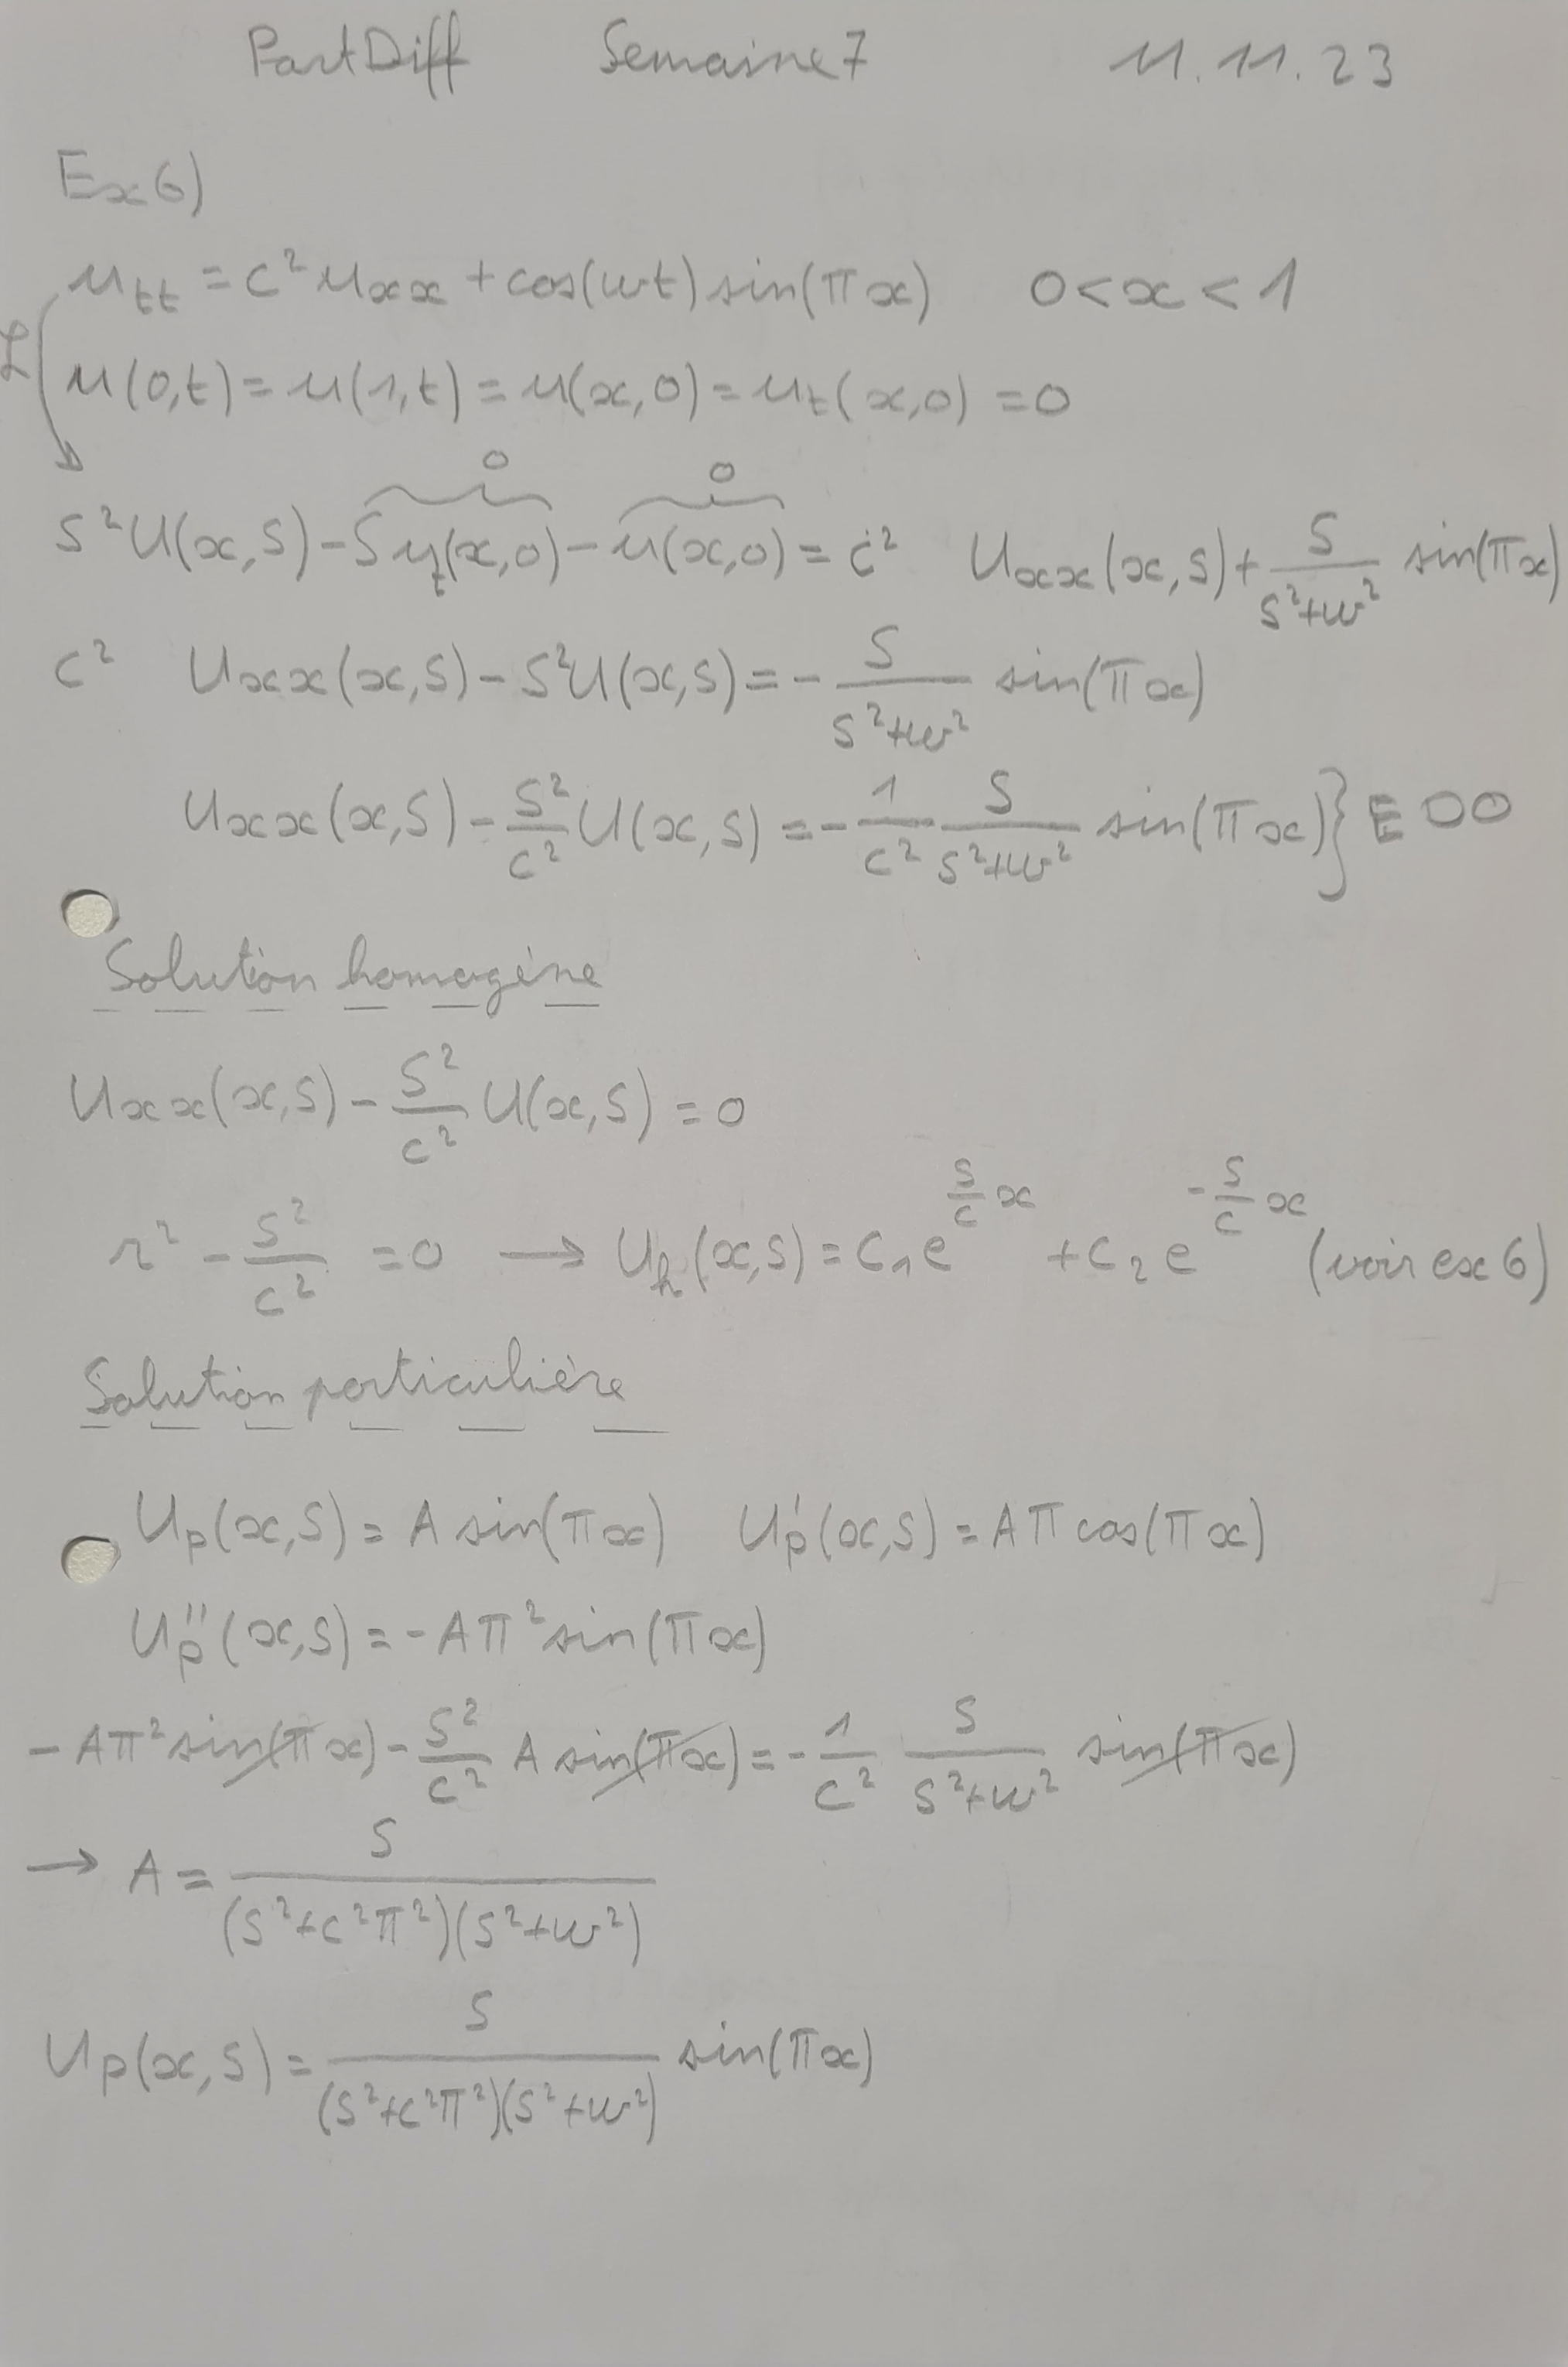
\includegraphics[height=\textheight-1cm, width=\columnwidth]{images/semaine7_exemple_laplace4.jpg}
\end{figure}
\begin{figure}[H]
    \centering
    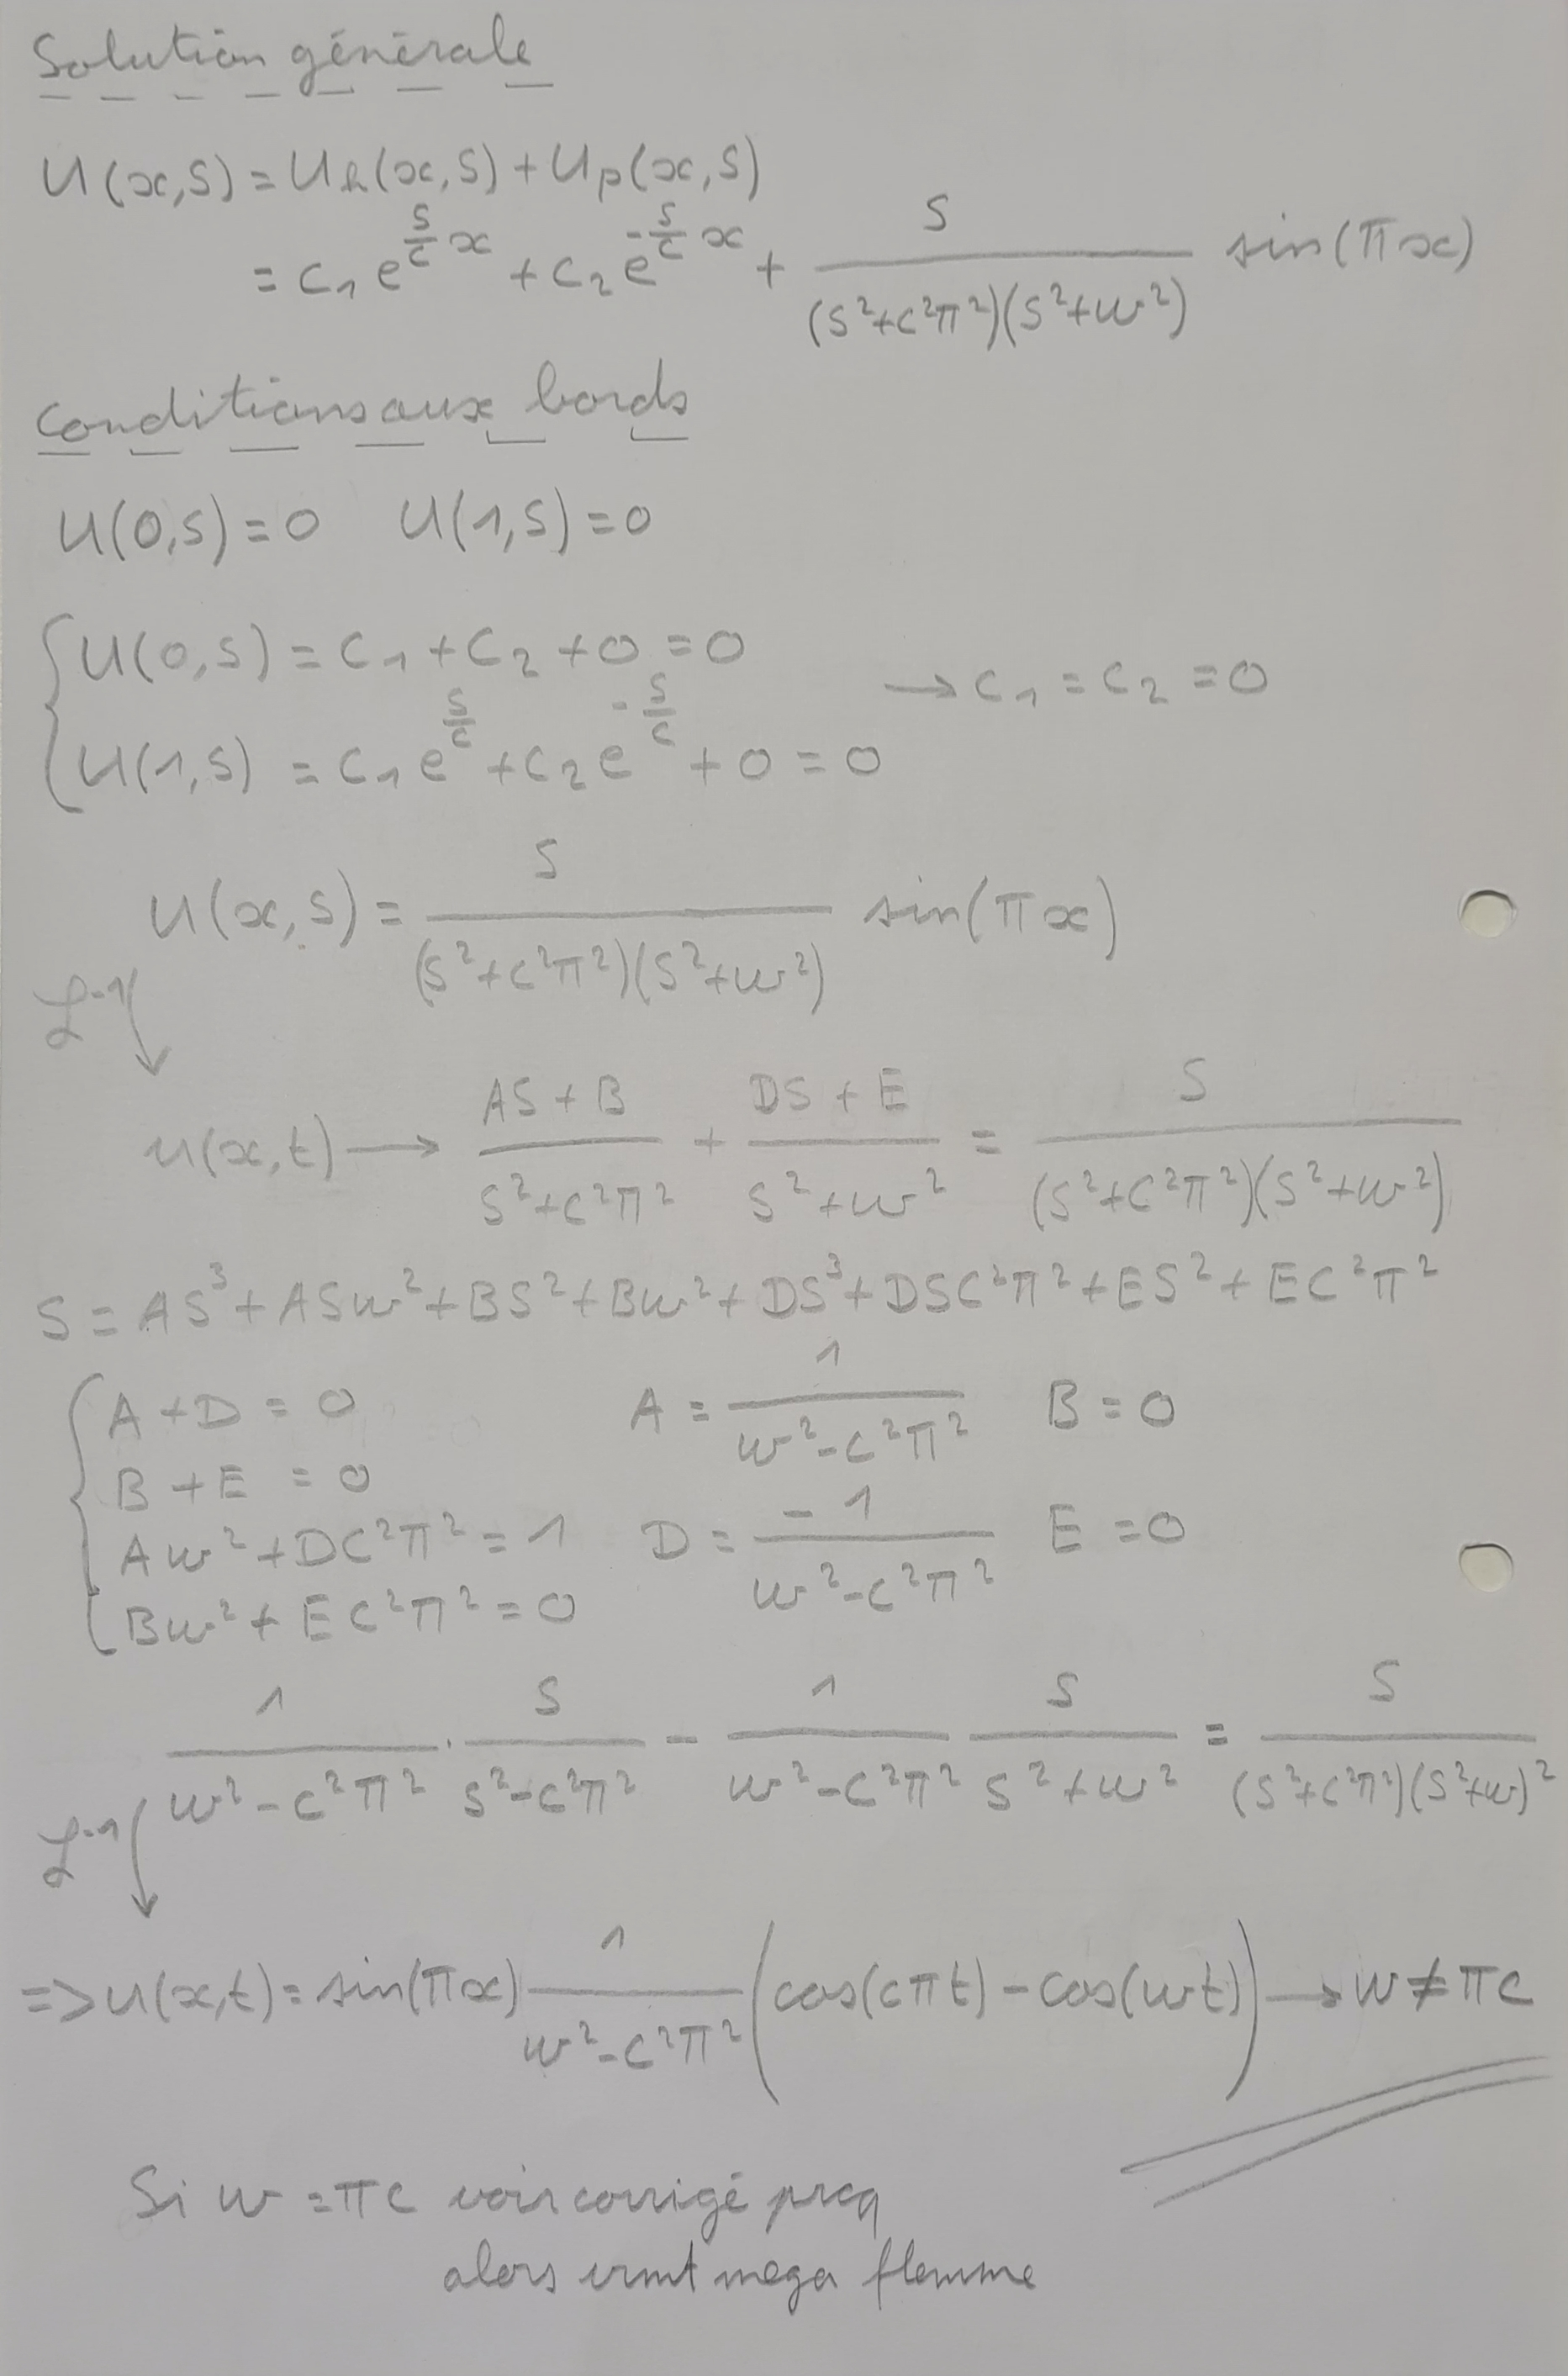
\includegraphics[height=\textheight, width=\columnwidth]{images/semaine7_exemple_laplace5.jpg}
\end{figure}
% \begin{figure}[H]
%     \centering
%     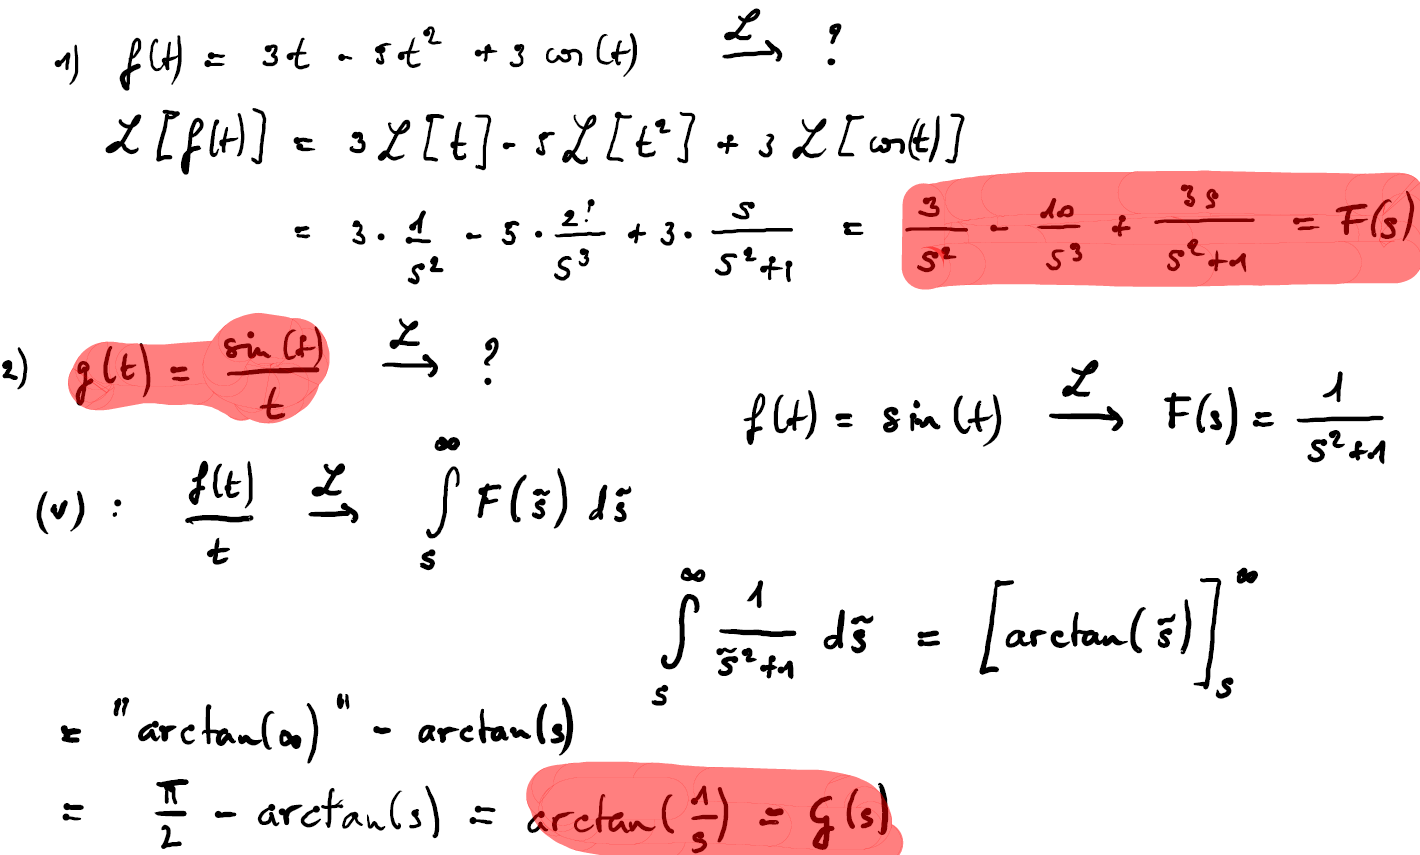
\includegraphics[width=\linewidth]{images/semaine7_exemple_laplace1.png}
% \end{figure}
% \begin{figure}[H]
%     \centering
%     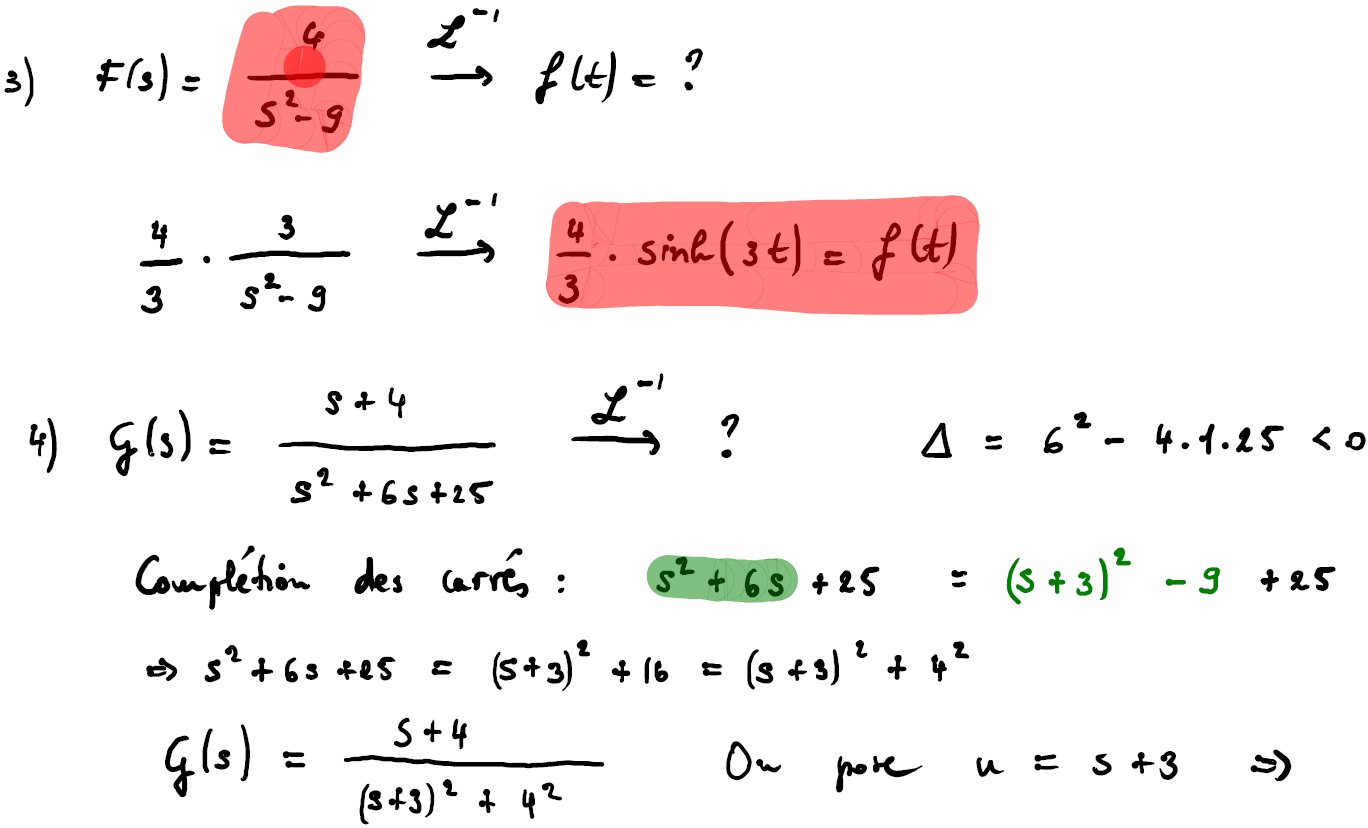
\includegraphics[width=\linewidth]{images/semaine7_exemple_laplace2.png}
% \end{figure}
% \begin{figure}[H]
%     \centering
%     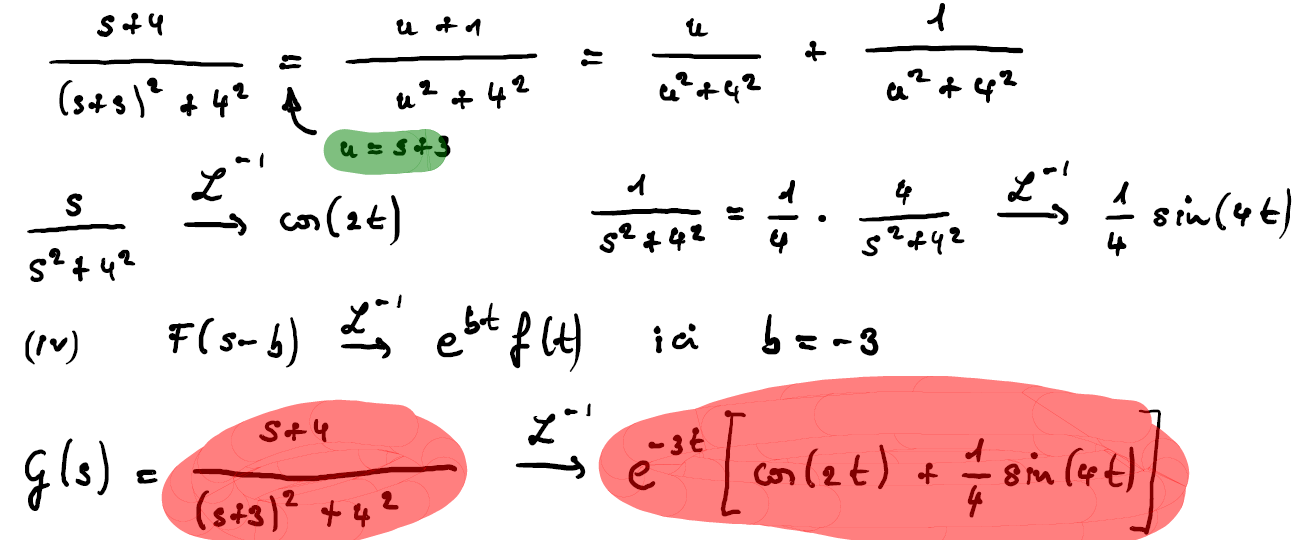
\includegraphics[width=\linewidth]{images/semaine7_exemple_laplace3.png}
% \end{figure}

    \subsection*{Méthode des différences finies}
\textbf{Principe:}\\
On veut discrétiser une fonction $u(x,y)$ sur un domaine $\Omega$ en utilisant un pas $h$.
\begin{subequations}
    \begin{equation*}
        \underbrace{-\Delta u(x,y)+c(x,y)u(x,y)}_{\mathcal{L}u}=f(x,y)
    \end{equation*}
    \begin{equation*}
        \mathcal{L}u=f\leftrightarrow \mathcal{L}_h\overrightarrow{u_h}=\overrightarrow{f_h}
    \end{equation*}
    \begin{equation*}
        \begin{pmatrix}
             &               & \\
             & \mathcal{L}_h & \\
             &               &
        \end{pmatrix}
        \begin{pmatrix}
            |                    \\
            \overrightarrow{u_h} \\
            |                    \\
        \end{pmatrix}
        =
        \begin{pmatrix}
            |                    \\
            \overrightarrow{f_h} \\
            |                    \\
        \end{pmatrix}
    \end{equation*}
\end{subequations}
\textbf{Discrétisation:}\\
Pour un pas $h=x_{i+1}-x_i=x_i-x_{i-1}$.\\
\underline{Décentré à droite (forward):}
% \begin{subequations}
%     \begin{equation*}
%         \frac{\mathrm{d}u}{\mathrm{d} x}\approx \frac{u(x_i+h)-u(x_i)}{h}\approx \frac{u_{i+1}-u_i}{h}
%     \end{equation*}
%     \begin{equation*}
%         \frac{\partial u}{\partial x}\approx \frac{u_{i+1,j}-u_{i,j}}{h_x}
%     \end{equation*}
%     \begin{equation*}
%         \frac{\partial u}{\partial y}\approx \frac{u_{i,j+1}-u_{i,j}}{h_y}
%     \end{equation*}
% \end{subequations}
\begin{empheq}[box=\fbox]{gather*}
    \frac{\mathrm{d}u}{\mathrm{d} x}\approx \frac{u(x_i+h)-u(x_i)}{h}\approx \frac{u_{i+1}-u_i}{h} \\
    \frac{\partial u}{\partial x}\approx \frac{u_{i+1,j}-u_{i,j}}{h_x}\\
    \frac{\partial u}{\partial y}\approx \frac{u_{i,j+1}-u_{i,j}}{h_y}
\end{empheq}
\underline{Décentré à gauche (backward):}
% \begin{subequations}
%     \begin{equation*}
%         \frac{\mathrm{d}u}{\mathrm{d} x}\approx \frac{u(x_i)-u(x_i-h)}{h}\approx \frac{u_{i}-u_{i-1}}{h}
%     \end{equation*}
%     \begin{equation*}
%         \frac{\partial u}{\partial x}\approx \frac{u_{i,j}-u_{i-1,j}}{h_x}
%     \end{equation*}
%     \begin{equation*}
%         \frac{\partial u}{\partial y}\approx \frac{u_{i,j}-u_{i,j-1}}{h_y}
%     \end{equation*}
% \end{subequations}
\begin{empheq}[box=\fbox]{gather*}
    \frac{\mathrm{d}u}{\mathrm{d} x}\approx \frac{u(x_i)-u(x_i-h)}{h}\approx \frac{u_{i}-u_{i-1}}{h} \\
    \frac{\partial u}{\partial x}\approx \frac{u_{i,j}-u_{i-1,j}}{h_x}\\
    \frac{\partial u}{\partial y}\approx \frac{u_{i,j}-u_{i,j-1}}{h_y}
\end{empheq}
\underline{Centré (différences finies):}
% \begin{subequations}
%     \begin{equation*}
%         \frac{\mathrm{d}u}{\mathrm{d} x}\approx \frac{u(x_i+h)-u(x_i-h)}{2h}\approx \frac{u_{i+1}-u_{i-1}}{2h}
%     \end{equation*}
%     \begin{equation*}
%         \frac{\partial u}{\partial x}\approx \frac{u_{i+1,j}-u_{i-1,j}}{2h_x}
%     \end{equation*}
%     \begin{equation*}
%         \frac{\partial u}{\partial y}\approx \frac{u_{i,j+1}-u_{i,j-1}}{2h_y}
%     \end{equation*}
% \end{subequations}
\begin{empheq}[box=\fbox]{gather*}
    \frac{\mathrm{d}u}{\mathrm{d} x}\approx \frac{u(x_i+h)-u(x_i-h)}{2h}\approx \frac{u_{i+1}-u_{i-1}}{2h} \\
    \frac{\partial u}{\partial x}\approx \frac{u_{i+1,j}-u_{i-1,j}}{2h_x}\\
    \frac{\partial u}{\partial y}\approx \frac{u_{i,j+1}-u_{i,j-1}}{2h_y}
\end{empheq}
\underline{Deuxième ordre:}
% \begin{subequations}
%     \begin{equation*}
%         \frac{\mathrm{d}^2u}{\mathrm{d} x^2}\approx \frac{u(x_i-h)-2u(x_i)+u(x_i+h)}{h^2}\approx \frac{u_{i-1}-2u_i+u_{i+1}}{h^2}
%     \end{equation*}
%     \begin{equation*}
%         \frac{\partial^2 u}{\partial x^2}\approx \frac{u_{i-1,j}-2u_{i,j}+u_{i+1,j}}{h_x^2}
%     \end{equation*}
%     \begin{equation*}
%         \frac{\partial^2 u}{\partial y^2}\approx \frac{u_{i,j-1}-2u_{i,j}+u_{i,j+1}}{h_y^2}
%     \end{equation*}
%     \begin{equation*}
%         \frac{\partial^2 u}{\partial x \partial y}\approx \frac{u_{i+1,j+1}-u_{i+1,j-1}-u_{i-1,j+1}+u_{i-1,j-1}}{4h_xh_y}
%     \end{equation*}
% \end{subequations}
\begin{empheq}[box=\fbox]{gather*}
    \frac{\mathrm{d}^2u}{\mathrm{d} x^2}\approx \frac{u(x_i-h)-2u(x_i)+u(x_i+h)}{h^2}\approx \frac{u_{i-1}-2u_i+u_{i+1}}{h^2} \\
    \frac{\partial^2 u}{\partial x^2}\approx \frac{u_{i-1,j}-2u_{i,j}+u_{i+1,j}}{h_x^2}\\
    \frac{\partial^2 u}{\partial y^2}\approx \frac{u_{i,j-1}-2u_{i,j}+u_{i,j+1}}{h_y^2}\\
    \frac{\partial^2 u}{\partial x \partial y}\approx \frac{u_{i+1,j+1}-u_{i+1,j-1}-u_{i-1,j+1}+u_{i-1,j-1}}{4h_xh_y}
\end{empheq}
\textbf{Exemple 1D:}\\
Soit le problème suivant:
\begin{equation*}
    \left\{
    \begin{aligned}
         & -u''(x)+c(x)u(x)=f(x)\quad \text{dans} \quad \Omega=(0,1) \\
         & u(0)=\alpha                                               \\
         & \lambda u(1)+u'(1)=g\quad (CB:Robin)                      \\
    \end{aligned}
    \right.
\end{equation*}
On sait que $x_1=0$ et donc que \colorbox{orange}{$u_1=\alpha$}. Pour les $x_i$ ont discrétise l'équation
différentielle:
\begin{gather*}
    -\left(\frac{u_{i-1}-2u_i+u_{i+1}}{h^2}\right)+c_iu_i=f_i\\
    -\frac{1}{h^2}u_{i-1}+\frac{1}{h^2}u_i\left(2+h^2c_i\right)-\frac{1}{h^2}u_{i+1}=fi\\
    \colorbox{green}{$\displaystyle\frac{1}{h^2}\left[-u_{i-1}+u_i(2+h^2c_i)-u_{i+1}\right]=f_i$}
\end{gather*}
On sait que $x_N=1$, discrétisée par le technique du point fictif la condition au bord de Robin:
\begin{subequations}
    \begin{equation*}
        \lambda u_N+\frac{u_{N+1}-u_{N-1}}{2h}=g
    \end{equation*}
    \begin{equation*}
        u_{N+1}=2h(g-\lambda u_N)+u_{N-1}
    \end{equation*}
\end{subequations}
En supposant que l'équation différentielle est valide aussi au bord $x_N=1$ on la discrétise:
\begin{equation*}
    -\left(\frac{u_{N-1}-2u_N+u_{N+1}}{h^2}\right)+c_Nu_N=f_N
\end{equation*}
Dans laquelle on substitue $u_{N+1}$:
\begin{gather*}
    -\left(\frac{u_{N-1}-2u_N+2h(g-\lambda u_N)+u_{N-1}}{h^2}\right)+c_Nu_N  =f_N              \\
    -\left(\frac{u_{N-1}-2u_N+2hg-2h\lambda u_N+u_{N-1}}{h^2}\right)+c_Nu_N  =f_N              \\
    -\frac{2}{h^2}u_{N-1}+\frac{1}{h^2}u_N\left(2+2h\lambda+h^2c_N\right)    =f_N+\frac{2g}{h} \\
    \colorbox{yellow}{$\frac{1}{h^2}\left[-2u_{N-1}+u_N(2+2h\lambda+h^2c_N)\right]              =f_N+\frac{2g}{h}$}
\end{gather*}
On obtient donc le système suivant:
\begin{gather*}
    \frac{1}{h^2}
    \resizebox{0.75\columnwidth}{!}{%
        $\left(\begin{tabular}{cccccc}
                \rowcolor{orange}$1$  & $0$        & $0$        & $0$      & $0$            & $0$                  \\
                \rowcolor{green} $-1$ & $2+h^2c_2$ & $-1$       & $0$      & $0$            & $0$                  \\
                \rowcolor{green}$0$   & $-1$       & $2+h^2c_3$ & $-1$     & $0$            & $0$                  \\
                \rowcolor{green}$0$   & $0$        & $0$        & $\ddots$ & $0$            & $0$                  \\
                \rowcolor{green}$0$   & $0$        & $0$        & $0$      & $2+h^2c_{N-1}$ & $-1$                 \\
                \rowcolor{yellow}$0$  & $0$        & $0$        & $0$      & $-2$           & $2+2h\lambda+h^2c_N$ \\
            \end{tabular}\right)$}%
    \cdot
    \left(\begin{smallmatrix}
            u_1    \\
            u_2    \\
            u_3    \\
            \vdots \\
            u_{N-1} \\
            u_N    \\
        \end{smallmatrix}\right)\\
    =
    \resizebox{0.2\columnwidth}{!}{% Add this line
        $\left(\begin{tabular}{c}
                \rowcolor{orange}$\frac{\alpha}{h^2}$ \\
                \rowcolor{green} $f_2$                \\
                \rowcolor{green} $f_3$                \\
                \rowcolor{green} $\vdots$             \\
                \rowcolor{green} $f_{N-1}$            \\
                \rowcolor{yellow} $f_N+\frac{2g}{h}$  \\
            \end{tabular}\right)$}% Add this line
\end{gather*}
\textbf{Exemple 2D:}\\
On veut trouver une approximation numérique de $-\Delta u=f(x,y)$ dans $\Omega=(0,1)\times(0,1)$.
Couvrir $\Omega$ avec un maillage régulier de pas $h_x=h_y=h$:
\begin{figure}[H]
    \centering
    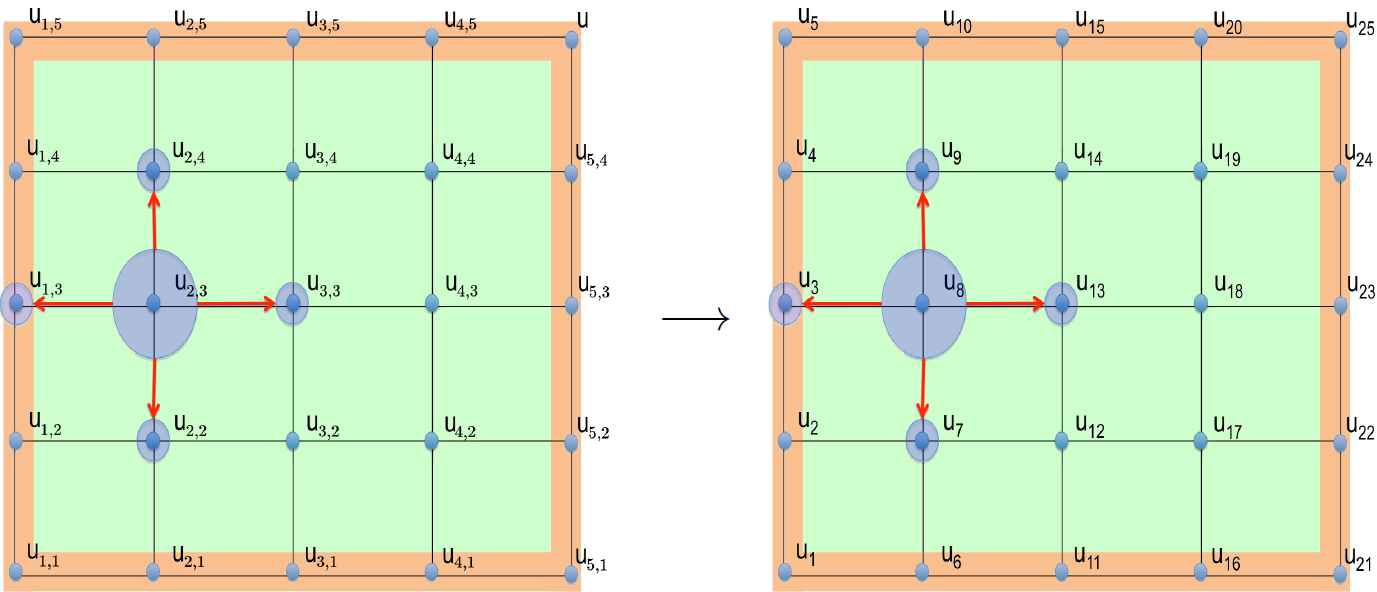
\includegraphics[width=\linewidth]{images/semaine9_diff_finies_2d.png}
\end{figure}
Approchée, l'équation différentielle devient:
\begin{equation*}
    -\Delta u(\overrightarrow{x_{i,j}})\approx\frac{1}{h_x^2}[-u_{i-1,j}+2u_{i,j}-u_{i+1,j}]+\frac{1}{h_y^2}[-u_{i,j-1}+2u_{i,j}-u_{i,j+1}]
\end{equation*}
Comme $h_x=h_y=h$:
\begin{equation*}
    -\Delta u(\overrightarrow{x_{i,j}})\approx\frac{1}{h^2}[4u_{i,j}-u_{i-1,j}-u_{i+1,j}-u_{i,j-1}-u_{i,j+1}]
\end{equation*}
En réecrivant $u_{i,j}\rightarrow u_l$, $l=1,\dots,N$. On a par exemple pour
$\overrightarrow{x}_{2,3}=\overrightarrow{x}_8$:
\begin{equation*}
    -\Delta u(\overrightarrow{x}_8)\approx\frac{1}{h^2}[4u_8-u_3-u_13-u_7-u_9]
\end{equation*}
C'est le stencil à 5 points:
\begin{equation*}
    \frac{1}{h^2}
    \begin{bmatrix}
        \cdot & -1 & \cdot \\
        -1    & 4  & -1    \\
        \cdot & -1 & \cdot \\
    \end{bmatrix}
\end{equation*}




    \subsection*{Analyse de convergence}
\textbf{Erreur de troncature}\\
L'erreur de troncature est l'erreur commise en remplaçant une dérivée par une différence finie:
\begin{equation*}
    \boxed{|e_h'(x_i)|=|u_h'(x_i)-u'(x_i)|\leq C\cdot h^p}
\end{equation*}
avec $p$ l'ordre du stencil (degré de la dérivée approchée).\\
\underline{Exemple:}\\
Pour déterminer l'erreur de troncature, on exprime le stencil grâce Taylor.
Pour un schéma centré $u'(x_i)$:
\begin{align*}
    u_{i+1}=u(x_i+h)= & u(x_i)+hu'(x_i)+\frac{h^2}{2}u''(x_i)                     \\
                      & +\frac{h^3}{6}u'''(x_i)+\frac{h^4}{24}u^{(4)}(x_i)+\cdots \\
    u_{i-1}=u(x_i-h)= & u(x_i)-hu'(x_i)+\frac{h^2}{2}u''(x_i)                     \\
                      & -\frac{h^3}{6}u'''(x_i)+\frac{h^4}{24}u^{(4)}(x_i)+\cdots \\
\end{align*}
et on soustraie les deux équations:
\begin{subequations}
    \begin{equation*}
        u_{i+1}-u_{i-1}=2hu'(x_i)+\frac{h^3}{3}u'''(x_i)+\cdots
    \end{equation*}
    \begin{equation*}
        u'(x_i)=\frac{u_{i+1}-u_{i-1}}{2h}-\frac{h^2}{6}u'''(x_i)+\cdots
    \end{equation*}
\end{subequations}
Ce qui donne l'erreur de troncature:
\begin{equation*}
    e_h'(x_i)\leq\underbrace{\frac{h^2}{6}u'''(x_i)}_C\cdot h^2
\end{equation*}
\textbf{Vitesse de couvergence (erreur à priori)}\\
% \begin{gather*}
%     ||(\overrightarrow{u})_h-\overrightarrow{u}_h||_{\infty}\leq C\cdot h^p\\
%     ||(\overrightarrow{u})_h-\overrightarrow{u}_h||_{\infty}\leq \underbrace{||\mathcal{L}_h^{-1}||_{\infty}}_{\leq C_S}\cdot \underbrace{||\mathcal{L}_h(\overrightarrow{u})_h-\mathcal{L}_h\overrightarrow{u}_h||_{\infty}}_{\kappa h^p}\leq C_S\kappa h^p
% \end{gather*}
\begin{empheq}[box=\fbox]{gather*}
    ||(\overrightarrow{u})_h-\overrightarrow{u}_h||_{\infty}\leq C\cdot h^p\\
    ||(\overrightarrow{u})_h-\overrightarrow{u}_h||_{\infty}\leq \underbrace{||\mathcal{L}_h^{-1}||_{\infty}}_{\leq C_S}\cdot \underbrace{||\mathcal{L}_h(\overrightarrow{u})_h-\mathcal{L}_h\overrightarrow{u}_h||_{\infty}}_{\kappa h^p}\leq C_S\kappa h^p
\end{empheq}
avec $C_S$ la stabilité et $\kappa h^p$ la consistance.




    \subsection*{Problèmes évolutifs}
\textbf{Méthode explicite:}
\begin{equation*}
    \boxed{\frac{\mathrm{d}\overrightarrow{u_h}(t_k)}{\mathrm{d}t}\approx \frac{\overrightarrow{u_h}(t_k+\tau)-\overrightarrow{u_h}(t_k)}{\tau}=\frac{\overrightarrow{u_h}^{(k+1)}-\overrightarrow{u_h}^{(k)}}{\tau}}
\end{equation*}
Puis faire Euler, Heun, Runge-Kutta (voir formulaire CompAlg).
Il faut que $\tau$ soit suffisamment petit pour que la méthode soit stable:
\begin{equation*}
    \tau\leq \frac{2}{\lambda_{max}}
\end{equation*}
$\lambda_{max}$ est la plus grande valeur propre de la matrice $A$ du problème de Cauchy.\\
\textbf{Méthode implicite:}
\begin{equation*}
    \boxed{\frac{\mathrm{d}\overrightarrow{u_h}(t_{k+1})}{\mathrm{d}t}\approx \frac{\overrightarrow{u_h}(t_{k+1})-\overrightarrow{u_h}(t_{k+1}-\tau)}{\tau}=\frac{\overrightarrow{u_h}^{(k+1)}-\overrightarrow{u_h}^{(k)}}{\tau}}
\end{equation*}
\textbf{Exemple:}\\
Soit le problème suivant:
\begin{figure}[H]
    \centering
    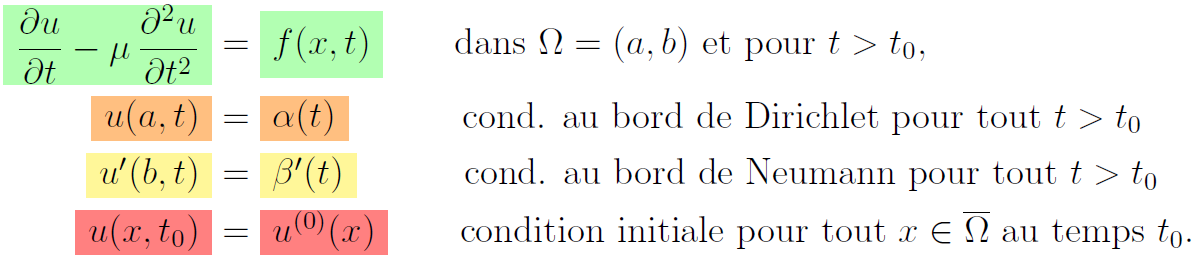
\includegraphics[width=\columnwidth]{images/semaine12_exemple_evolutif1.png}
\end{figure}
\underline{Semi-discrétisation en espace:}\\
Discrétiser l'équation par les différences finies centrées en espace et préparer le
problème de Cauchy pour l'itération en temps:
\begin{figure}[H]
    \centering
    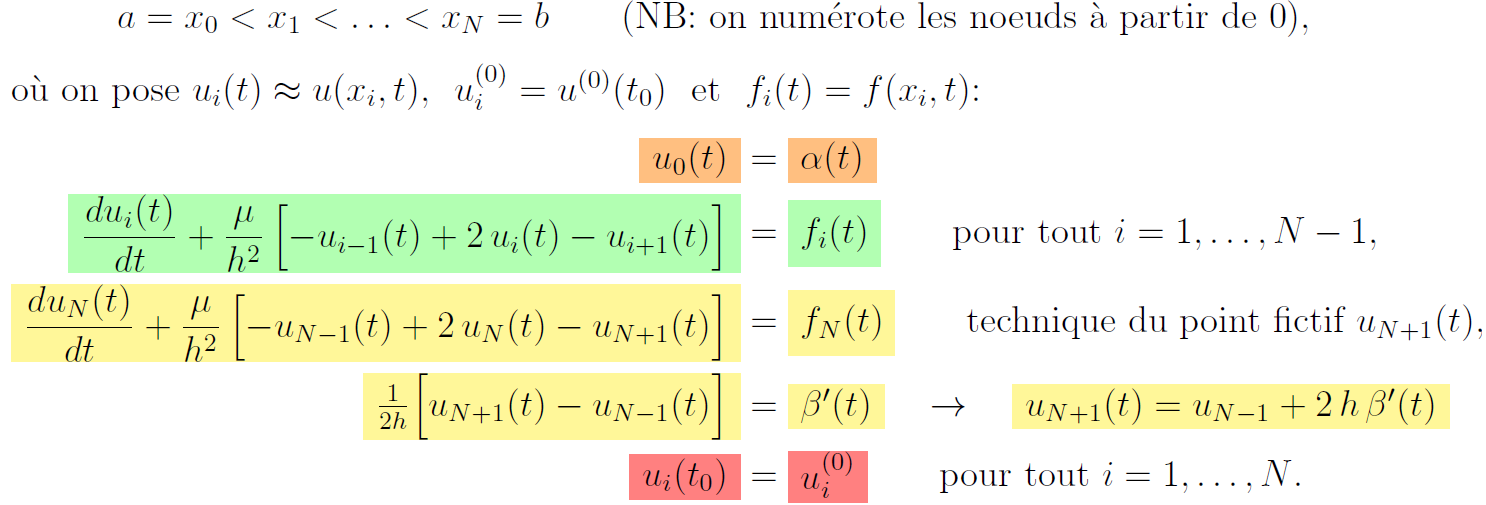
\includegraphics[width=\columnwidth]{images/semaine12_exemple_evolutif2.png}
\end{figure}
Eliminer la valeur fictive $u_{N+1}(t)$ et la valeur de la condition au bord
$u_0(t)=\alpha(t)$:
\begin{figure}[H]
    \centering
    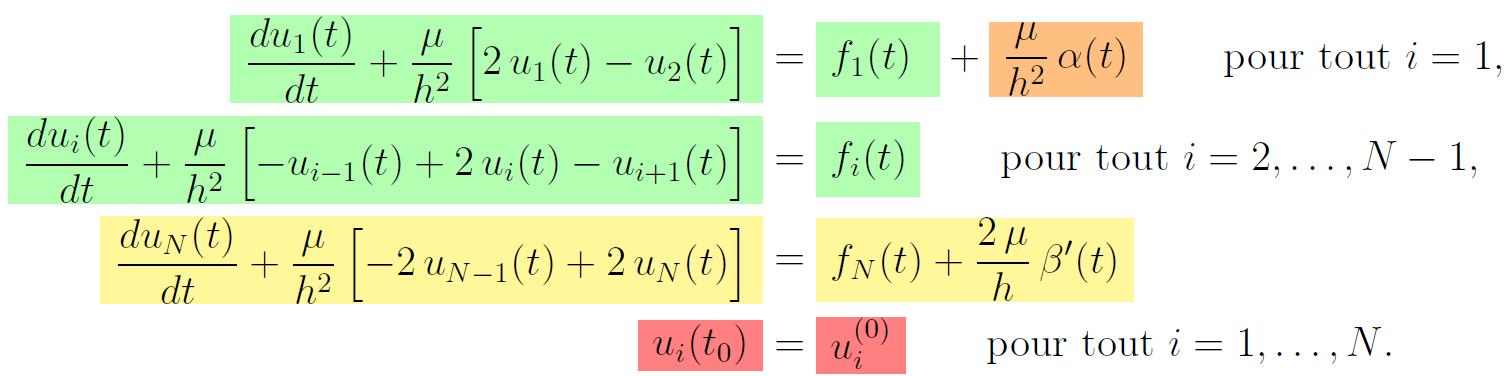
\includegraphics[width=\columnwidth]{images/semaine12_exemple_evolutif3.png}
\end{figure}
Sous forme matricielle:
\begin{figure}[H]
    \centering
    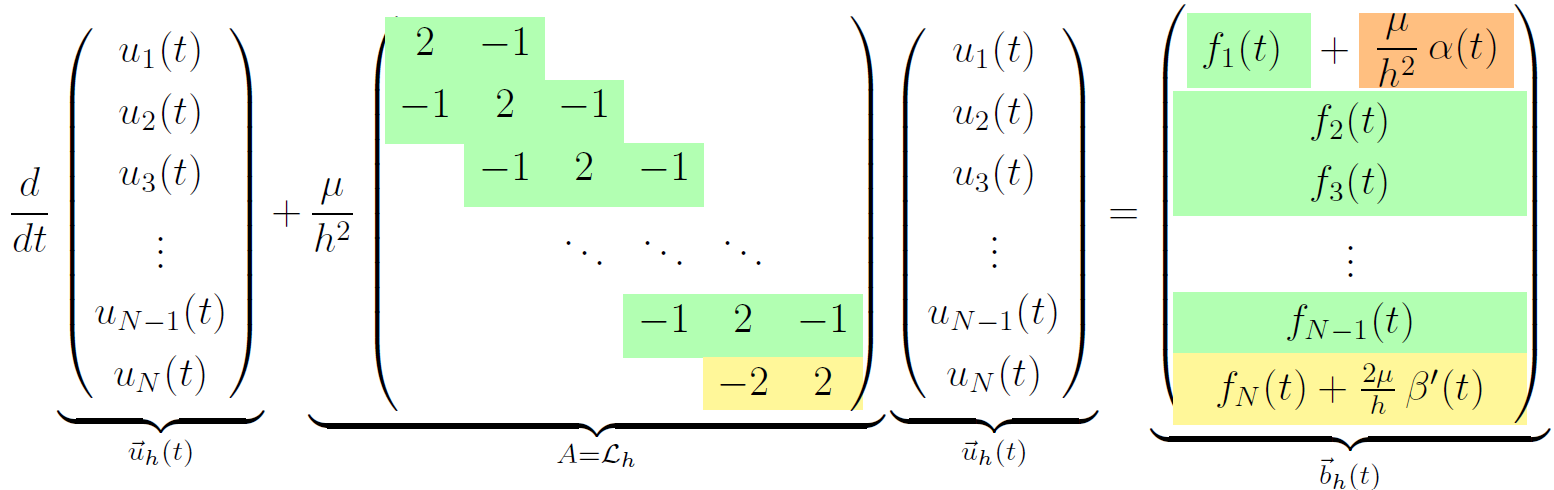
\includegraphics[width=\columnwidth]{images/semaine12_exemple_evolutif4.png}
\end{figure}
\begin{figure}[H]
    \centering
    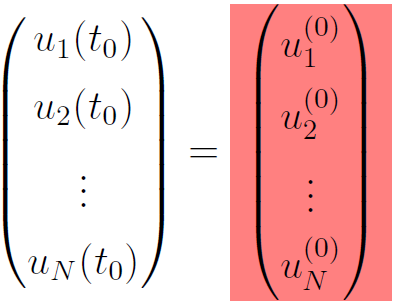
\includegraphics[width=0.3\columnwidth]{images/semaine12_exemple_evolutif5.png}
\end{figure}
Pour obtenir le \underline{problème de Cauchy}, on isole $\frac{\mathrm{d}\overrightarrow{u_h}(t)}{\mathrm{d}t}$
\begin{equation*}
    \boxed{\frac{\mathrm{d}\overrightarrow{u_h}(t)}{\mathrm{d}t}=\underbrace{\overrightarrow{b_h}(t)-A\overrightarrow{u_h}(t)}_{\overrightarrow{f}(t,\overrightarrow{u_h}(t))}}
\end{equation*}
\underline{Discrétisation:}\\
connaisant la solution exacte $u(x,t)$:
\begin{equation*}
    u(x,t)=e^{-\mu t}x\cos(x)+e^{-\frac{4}{9}\pi^2\mu t}\sin(\frac{3\pi}{2}x)
\end{equation*}
On peut calculer $u_i(0)$:
\begin{equation*}
    u_i(0)=u(x_i,0)=x_i\cos(x_i)+\sin(\frac{3\pi}{2}x_i)
\end{equation*}
\underline{Résolution numérique:}\\
Avec Euler, Heun, Runge-Kutta on itère en temps, dans ce cas on prend Euler:
\begin{equation*}
    \overrightarrow{u_h}^{(0)}=
    \begin{pmatrix}
        x_1\cos(x_1)+\sin(\frac{3\pi}{2}x_1) \\
        x_2\cos(x_2)+\sin(\frac{3\pi}{2}x_2) \\
        \vdots                               \\
        x_N\cos(x_N)+\sin(\frac{3\pi}{2}x_N) \\
    \end{pmatrix}
\end{equation*}


    \columnbreak
    \subsection*{Méthode des volumes finis}
\textbf{Flux:}\\
\underline{Convectif:}
\begin{equation*}
    \boxed{\int_{\partial C_{ij}}(\overrightarrow{v}\space u)\cdot \overrightarrow{n}\space\mathrm{d}S\approx \phi_{ij}^C(u)=|\partial C_{ij}|(\overrightarrow{v_{ij}}\cdot\overrightarrow{n_{ij}})\cdot u_{ij}}
\end{equation*}
\underline{Diffusif:}
\begin{equation*}
    \boxed{\int_{\partial C_{ij}}(\mu \nabla u)\cdot \overrightarrow{n}\space\mathrm{d}S\approx \phi_{ij}^D(u)=|\partial C_{ij}|\frac{\mu}{l_{ij}}(u_j-u_i)}
\end{equation*}
% \textbf{Schéma:}
% \begin{equation*}
%     \boxed{\frac{\mathrm{d}u_i}{\mathrm{d}t}=\frac{1}{V_i}\sum_{j\in\mathcal{N}_i}(\phi_{ij}^C(u)+\phi_{ij}^D(u))}
% \end{equation*}
\textbf{Création du maillage (diagramme de Voronoi):}\\
\begin{figure}[H]
    \centering
    \begin{minipage}{0.49\columnwidth}
        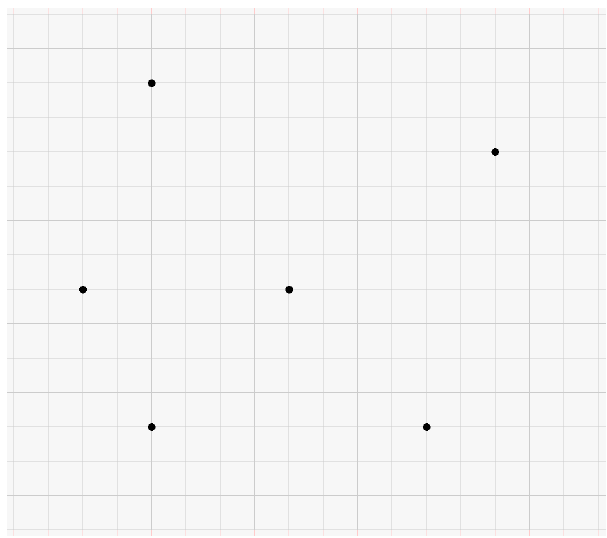
\includegraphics[width=\columnwidth]{images/semaine13_maillage1.png}
    \end{minipage}\hfill
    \begin{minipage}{0.49\columnwidth}
        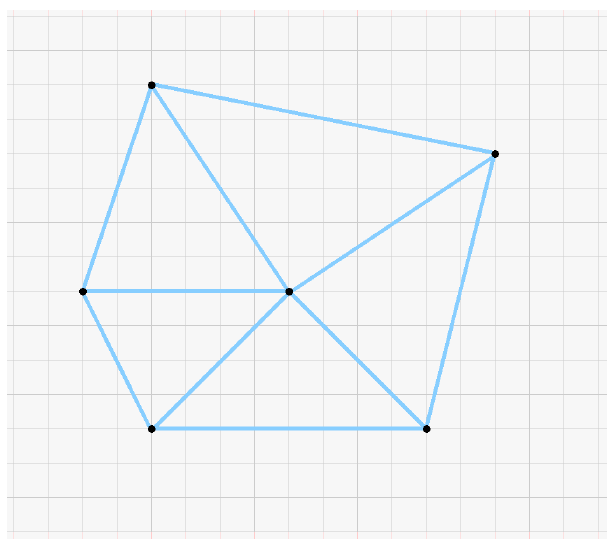
\includegraphics[width=\columnwidth]{images/semaine13_maillage2.png}
    \end{minipage}\hfill
    \begin{minipage}{0.49\columnwidth}
        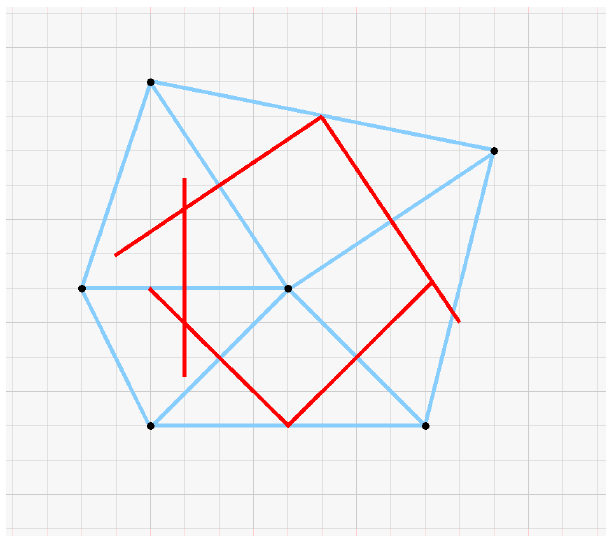
\includegraphics[width=\columnwidth]{images/semaine13_maillage3.png}
    \end{minipage}\hfill
    \begin{minipage}{0.49\columnwidth}
        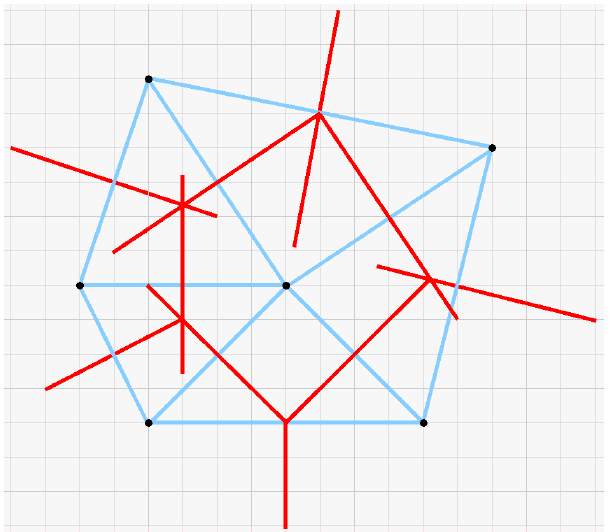
\includegraphics[width=\columnwidth]{images/semaine13_maillage4.png}
    \end{minipage}\hfill
    \begin{minipage}{0.5\columnwidth}
        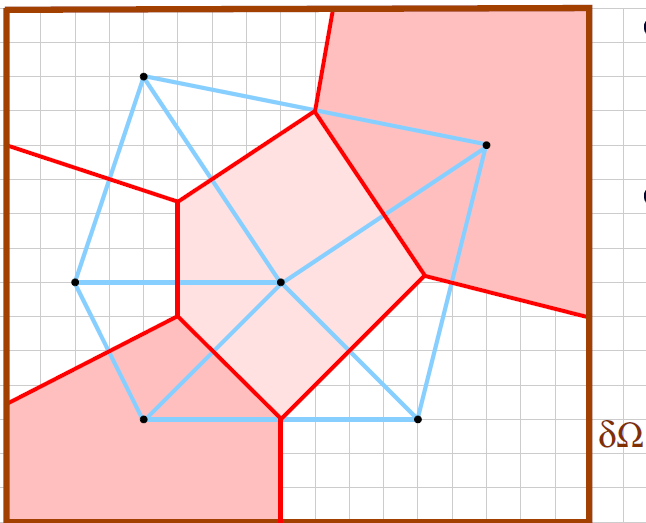
\includegraphics[width=\columnwidth]{images/semaine13_maillage5.png}
    \end{minipage}
\end{figure}

\end{multicols*}
\end{document}